\documentclass[a4paper, twoside, titlepage]{article}

\def\ssver{1.0.0}

% ====   Packages   ====
\usepackage[left=1cm, right=1cm, top=1cm, bottom=2cm]{geometry}
\usepackage[hyperindex]{hyperref}
\usepackage{makeidx}
\usepackage{pdfpages}
\usepackage{fancyhdr}
\usepackage{graphicx}
\usepackage{adjustbox}
\usepackage{multicol}
\usepackage{totcount}
\usepackage{xcolor}

% ====   Index   ====
\makeindex

% ====   Counters   ====
\newtotcounter{songcount}
\newtotcounter{psalmcount}
\definecolor{title dark}{HTML}{7E73A7}

% ====   Footer   ====
\pagestyle{fancy}
\fancyhf{}
\cfoot{{\small\thepage} \\ v{\ssver}}
\renewcommand{\headrulewidth}{0pt}

\makeatletter

% ====   Verse   ====
\renewcommand{\verse}{\@versei}
\newcommand{\@versei}{\@ifnextchar\end{\@verseend}{\@verseii}} % chktex 10
\newcommand{\@verseii}[1]{#1\par\@versei}
\newcommand{\@verseend}[1]{\vskip1em}

% ====   Chorus   ====
\newcommand{\chorus}{\@chorusi}
\newcommand{\@chorusi}{\@ifnextchar\end{\@chorusend}{\@chorusii}} % chktex 10
\newcommand{\@chorusii}[1]{\quad\textit{#1}\par\@chorusi}
\newcommand{\@chorusend}[1]{\vskip1em}

% ====   Bridge   ====
\newcommand{\bridge}{\@bridgei}
\newcommand{\@bridgei}{\@ifnextchar\end{\@bridgeend}{\@bridgeii}} % chktex 10
\newcommand{\@bridgeii}[1]{\textit{#1}\par\@bridgei}
\newcommand{\@bridgeend}[1]{\vskip1em}

\makeatother

% ====   Song   ====
\newenvironment{song}[1]%
{%
    \begin{minipage}[t]{0.94\columnwidth}{\stepcounter{songcount}\textbf{\large #1}\index{#1}}%
        \par\vspace{2pt}
}%
{%
    \end{minipage}%
    \vspace{2em}%
}

% ====   Psalm   ====
\newenvironment{psalm}[2]%
{%
    \begin{minipage}[t]{0.94\columnwidth}%
        \begin{center}{\stepcounter{psalmcount}\textbf{\large #1}\index{#1}{\normalsize #2}}%
            \par\vspace{2pt}
}%
{%
        \end{center}%
    \end{minipage}%
    \vspace{2em}%
}%

% ====   Utitilty Commands   ====
\newcommand{\extra}[1]{\textit{\normalsize (#1)}}
\renewcommand{\sp}{\textit{\normalsize (Sing Psalms)}}
\newcommand{\tr}{\textit{\normalsize (Scottish Psalter)}}
\newcommand{\LORD}{\textsc{Lord}}
\newcommand{\cp}[1]{{\tiny\ttfamily#1}}

% ====   Document   ====
\begin{document}
\sffamily

\begin{titlepage}
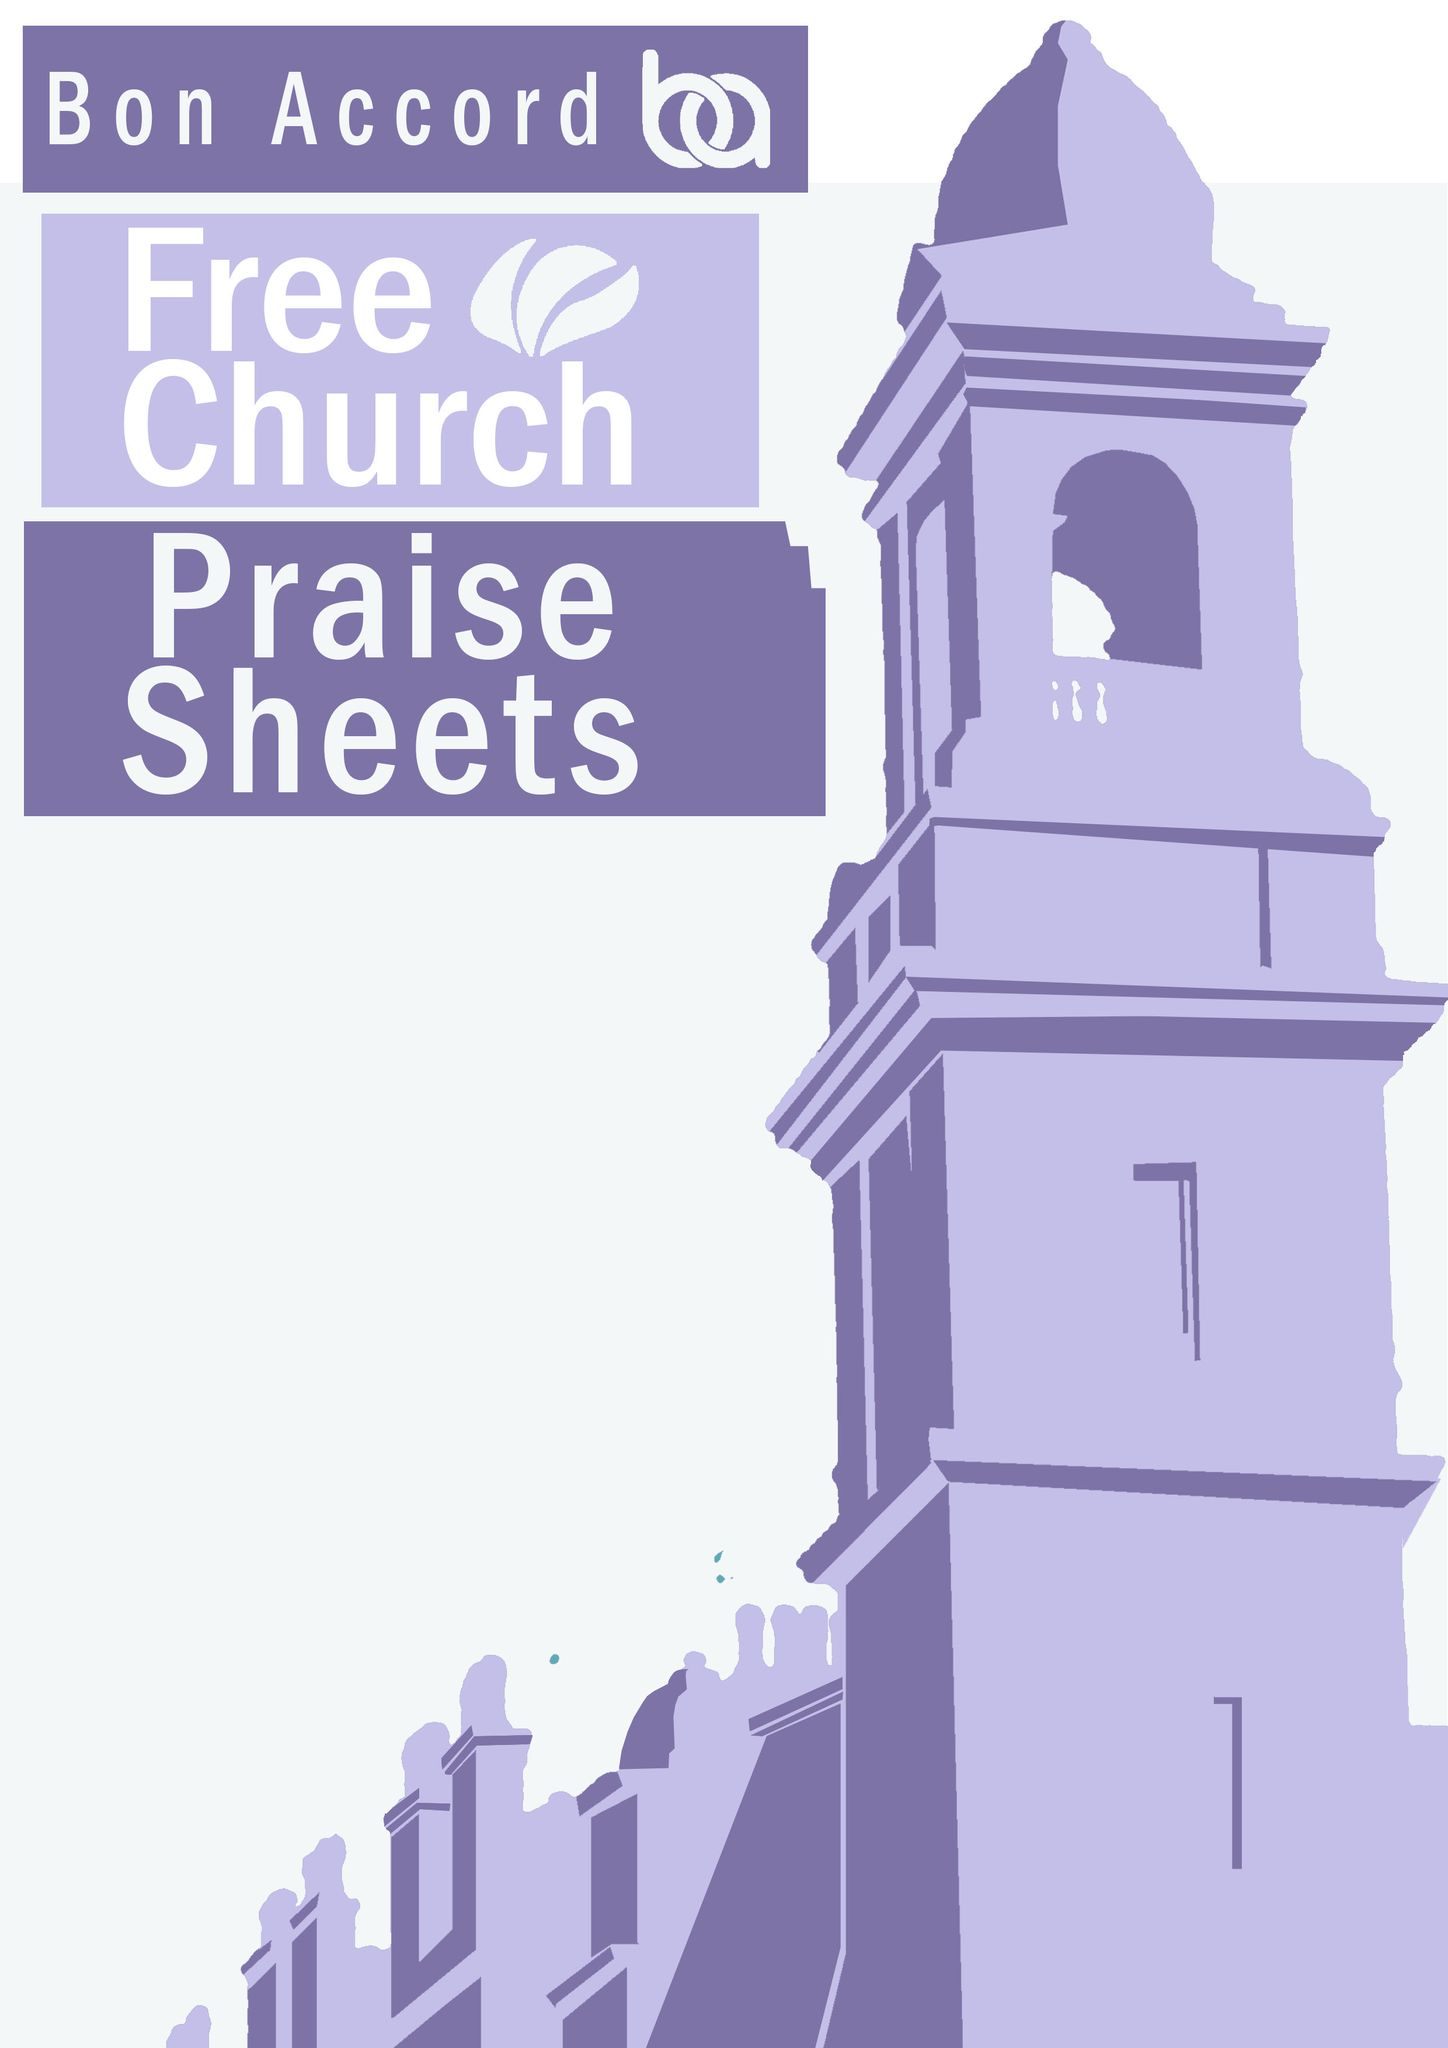
\includepdf{./titleimage.jpg}
\end{titlepage}

\setcounter{page}{2}  % Make title page, page 1
\printindex
\begin{multicols}{2}
\raggedcolumns{}

% ====   Abide with Me   ====
\begin{song}{Abide with Me}
    \verse
    {Abide with me: fast falls the eventide;}
    {the darkness deepens; Lord, with me abide.}
    {When other helpers fail and comforts flee,}
    {Help of the helpless, O abide with me.}
    \end
    \verse
    {Swift to its close ebbs out life's little day;}
    {earth's joys grow dim, its glories pass away,}
    {Change and decay in all around I see –}
    {O thou who changest not, abide with me.}
    \end
    \verse
    {I need thy presence every passing hour,}
    {What but thy grace can foil the tempter's power?}
    {Who like thyself my guide and strength can be?}
    {Through cloud and sunshine, O abide with me.}
    \end
    \verse
    {I fear no foe with thee at hand to bless,}
    {ills have no weight, and tears no bitterness,}
    {Where is death's sting? Where, grave, thy victory?}
    {I triumph still, if thou abide with me.}
    \end
\end{song}

% ====   Abide With Me (Eventide)   ====
\begin{song}{Abide With Me (Eventide)}
    \verse
    {Abide with me fast falls the eventide}
    {The darkness deepens Lord with me abide}
    {When other helpers fail and comforts flee}
    {Help of the helpless O abide with me}
    \end
    \verse
    {Swift to its close ebbs out life's little day}
    {Earth's joys grow dim its glories pass away}
    {Change and decay in all around I see}
    {O Thou who changest not abide with me}
    \end
    \verse
    {I need Thy presence ev'ry passing hour}
    {What but Thy grace can foil the tempter's pow'r}
    {Who like Thyself my Guide and Stay can be}
    {Through cloud and sunshine O abide with me}
    \end
    \verse
    {I fear no foe with Thee at hand to bless}
    {Ills have no weight and tears no bitterness}
    {Where is death's sting where grave thy victory}
    {I triumph still if Thou abide with me}
    \end
    \verse
    {Hold Thou Thy cross before my closing eyes}
    {Shine through the gloom and point me to the skies}
    {Heav'n's morning breaks}
    {And earth's vain shadows flee}
    {In life in death O Lord abide with me}
    \end
\end{song}

% ====   Across The Lands   ====
\begin{song}{Across The Lands}
    \verse
    {You're the Word of God the Father}
    {From before the world began,}
    {Every star and every planet}
    {Has been fashioned by Your hand.}
    \end
    \verse
    {All creation holds together}
    {By the power of Your voice,}
    {Let the skies declare Your glory;}
    {Let the land and seas rejoice!}
    \end
    \chorus
    {You're the Author of creation,}
    {You're the Lord of every man;}
    {And Your cry of love rings out}
    {Across the lands.}
    \end
    \verse
    {Yet You left the gaze of angels,}
    {Came to seek and save the lost,}
    {And exchanged the joy of heaven}
    {For the anguish of a cross.}
    \end
    \verse
    {With a prayer You fed the hungry,}
    {With a word You stilled the sea;}
    {Yet how silently You suffered}
    {That the guilty may go free!}
    \end
    \chorus
    {You're the Author of creation,}
    {You're the Lord of every man;}
    {And Your cry of love rings out}
    {Across the lands.}
    \end
    \verse
    {With a shout You rose victorious,}
    {Wresting victory from the grave,}
    {And ascended into heaven,}
    {Leading captives in Your way.}
    \end
    \verse
    {Now You stand before the Father,}
    {Interceding for Your own;}
    {From each tribe and tongue and nation,}
    {You are leading sinners home!}
    \end
    \chorus
    {You're the Author of creation,}
    {You're the Lord of every man;}
    {And Your cry of love rings out}
    {Across the lands.}
    \end
\end{song}

% ====   All Creatures of our God and King   ====
\begin{song}{All Creatures of our God and King}
    \verse
    {All creatures of our God and King}
    {Lift up your voice and with us sing}
    {Alleluia alleluia}
    {Thou burning sun with golden beam}
    {Thou silver moon with softer gleam}
    \end
    \chorus
    {O praise Him O praise Him}
    {Alleluia alleluia alleluia}
    \end
    \verse
    {Thou rushing wind that art so strong}
    {Ye clouds that sail in heaven along}
    {O praise Him alleluia}
    {Thou rising morn in praise rejoice}
    {Ye lights of evening find a voice}
    \end
    \chorus
    {O praise Him O praise Him}
    {Alleluia alleluia alleluia}
    \end
    \verse
    {And all ye men of tender heart}
    {Forgiving others take your part}
    {O sing ye alleluia}
    {Ye who long pain and sorrow bear}
    {Praise God and on Him cast your care}
    \end
    \chorus
    {O praise Him O praise Him}
    {Alleluia alleluia alleluia}
    \end
    \verse
    {Let all things their Creator bless}
    {And worship Him in humbleness}
    {O praise Him alleluia}
    {Praise, praise the Father, praise the Son}
    {And praise the Spirit, Three in One}
    \end
    \chorus
    {O praise Him O praise Him}
    {Alleluia alleluia alleluia}
    \end
\end{song}

% ====   All Glory Be To Christ   ====
\begin{song}{All Glory Be To Christ}
    \verse
    {Should nothing of our efforts stand}
    {No legacy survive}
    {Unless the Lord does raise the house}
    {In vain its builders strive}
    \end
    \verse
    {To you who boast tomorrow’s gain}
    {Tell me what is your life}
    {A mist that vanishes at dawn}
    {All glory be to Christ}
    \end
    \chorus
    {All glory be to Christ our king}
    {All glory be to Christ}
    {His rule and reign we’ll ever sing}
    {All glory be to Christ}
    \end
    \verse
    {His will be done His kingdom come}
    {On earth as is above}
    {Who is Himself our daily bread}
    {Praise Him the Lord of love}
    \end
    \verse
    {Let living water satisfy}
    {The thirsty without price}
    {We’ll take a cup of kindness yet}
    {All glory be to Christ}
    \end
    \chorus
    {All glory be to Christ our king}
    {All glory be to Christ}
    {His rule and reign we’ll ever sing}
    {All glory be to Christ}
    \end
    \verse
    {When on the day the great I Am}
    {The faithful and the true}
    {The Lamb who was for sinners slain}
    {Is making all things new}
    \end
    \verse
    {Behold our God shall live with us}
    {And be our steadfast light}
    {And we shall e'er his people be}
    {All glory be to Christ}
    \end
    \chorus
    {All glory be to Christ our king}
    {All glory be to Christ}
    {His rule and reign we’ll ever sing}
    {All glory be to Christ}
    \end
\end{song}

% ====   Amazing Grace   ====
\begin{song}{Amazing Grace}
    \verse
    {Amazing grace how sweet the sound}
    {That saved a wretch like me}
    {I once was lost but now am found}
    {Was blind but now I see}
    \end
    \verse
    {'Twas grace that taught my heart to fear}
    {And grace my fears relieved}
    {How precious did that grace appear}
    {The hour I first believed}
    \end
    \verse
    {The Lord has promised good to me,}
    {his word my hope secures;}
    {he will my shield and portion be}
    {as long as life endures}
    \end
    \verse
    {Through many dangers toils and snares}
    {I have already come}
    {'Tis grace has brought me safe thus far}
    {And grace will lead me home}
    \end
    \verse
    {Yea when this flesh and heart shall fail}
    {And mortal life shall cease}
    {I shall possess within the veil}
    {A life of joy and peace}
    \end
    \verse
    {When we've been there ten thousand years}
    {Bright shining as the sun}
    {We've no less days to sing God's praise}
    {Than when we've first begun}
    \end
\end{song}

% ====   Amazing Grace (My Chains Are Gone)   ====
\begin{song}{Amazing Grace (My Chains Are Gone)}
    \verse
    {Amazing grace how sweet the sound}
    {That saved a wretch like me}
    {I once was lost but now I'm found}
    {Was blind but now I see}
    \end
    \verse
    {'Twas grace that taught my heart to fear}
    {And grace my fears relieved}
    {How precious did that grace appear}
    {The hour I first believed}
    \end
    \chorus
    {My chains are gone I've been set free}
    {My God my Savior has ransomed me}
    {And like a flood His mercy rains}
    {Unending love amazing grace}
    \end
    \verse
    {The Lord has promised good to me}
    {His word my hope secures}
    {He will my shield and portion be}
    {As long as life endures}
    \end
    \verse
    {The earth shall soon dissolve like snow}
    {The sun forbear to shine}
    {But God who called me here below}
    {Will be forever mine}
    {Will be forever mine}
    {You are forever mine}
    \end
\end{song}

% ====   And Can It Be   ====
\begin{song}{And Can It Be}
    \verse
    {And can it be that I should gain}
    {An int'rest in the Saviour's blood?}
    {Died He for me, who caused His pain?}
    {For me, who Him to death pursued?}
    {Amazing love! how can it be}
    {That Thou, my God, should die for me?}
    \end
    \chorus
    {Bold I approach th'eternal throne,}
    {And claim the crown, through Christ my own.}
    \end
    \verse
    {'Tis mystery all! Th'Immortal dies!}
    {Who can explore His strange design?}
    {In vain the firstborn seraph tries}
    {To sound the depths of love divine!}
    {'Tis mercy all! let earth adore,}
    {Let angel minds inquire no more.}
    \end
    \chorus
    {Bold I approach th'eternal throne,}
    {And claim the crown, through Christ my own.}
    \end
    \verse
    {He left His Father's throne above,}
    {So free, so infinite His grace;}
    {Emptied Himself of all but love,}
    {And bled for Adam's helpless race;}
    {'Tis mercy all, immense and free;}
    {For, O my God, it found out me.}
    \end
    \chorus
    {Bold I approach th'eternal throne,}
    {And claim the crown, through Christ my own.}
    \end
    \verse
    {Long my imprisoned spirit lay}
    {Fast bound in sin and nature's night;}
    {Thine eye diffused a quick'ning ray,}
    {I woke, the dungeon flamed with light;}
    {My chains fell off, my heart was free;}
    {I rose, went forth and followed Thee.}
    \end
    \chorus
    {Bold I approach th'eternal throne,}
    {And claim the crown, through Christ my own.}
    \end
    \verse
    {No condemnation now I dread;}
    {Jesus, and all in Him is mine!}
    {Alive in Him, my living Head,}
    {And clothed in righteousness divine,}
    {Bold I approach th'eternal throne,}
    {And claim the crown, through Christ my own.}
    \end
    \chorus
    {Bold I approach th'eternal throne,}
    {And claim the crown, through Christ my own.}
    \end
\end{song}

% ====   Be Still   ====
\begin{song}{Be Still}
    \verse
    {Be still for the presence of the Lord}
    {The Holy One is here}
    {Come bow before Him now}
    {With reverence and fear}
    \end
    \verse
    {In Him no sin is found}
    {We stand on holy ground}
    {Be still for the presence of the Lord}
    {The Holy One is here}
    \end
    \verse
    {Be still for the glory of the Lord}
    {Is shining all around}
    {He burns with holy fire}
    {With splendour He is crowned}
    \end
    \verse
    {How awesome is the sight}
    {Our radiant King of light}
    {Be still for the glory of the Lord}
    {Is shining all around}
    \end
    \verse
    {Be still for the power of the Lord}
    {Is moving in this place}
    {He comes to cleanse and heal}
    {To minister His grace}
    \end
    \verse
    {No work too hard for Him}
    {In faith receive from Him}
    {Be still for the power of the Lord}
    {Is moving in this place}
    \end
\end{song}

% ====   Be Thou My Vision   ====
\begin{song}{Be Thou My Vision}
    \verse
    {Be thou my vision, O Lord of my heart;}
    {naught be all else to me, save that thou art.}
    {Thou my best thought, by day or by night,}
    {waking or sleeping, thy presence my light.}
    \end
    \verse
    {Be Thou my wisdom, Thou my true Word;}
    {I ever with Thee, Thou with me, Lord;}
    {Thou my great Father, and I Thy true son;}
    {Thou in me dwelling, and I with Thee one.}
    \end
    \verse
    {Be Thou my battle-shield, sword for the fight,}
    {be Thou my dignity, Thou my delight.}
    {Thou my soul’s shelter, Thou my high tower:}
    {raise Thou me heavenward, O Power of my power.}
    \end
    \verse
    {Riches I need not, nor man's empty praise,}
    {Thou mine inheritance, now and always:}
    {Thou and Thou only, first in my heart,}
    {High King of heaven, my treasure Thou art.}
    \end
    \verse
    {High King of heaven, after victory won,}
    {may I reach heaven’s joys, O bright heaven’s Sun!}
    {Heart of my own heart, whatever befall,}
    {still be my vision, O ruler of all.}
    \end
\end{song}

% ====   Before The Throne of God Above   ====
\begin{song}{Before The Throne of God Above}
    \verse
    {Before the throne of God above}
    {I have a strong and perfect plea}
    {A great High Priest whose name is Love}
    {Who ever lives and pleads for me}
    \end
    \verse
    {My name is graven on His hands}
    {My name is written on His heart}
    {I know that while in heav'n He stands}
    {No tongue can bid me thence depart}
    {No tongue can bid me thence depart}
    \end
    \verse
    {When Satan tempts me to despair}
    {And tells me of the guilt within}
    {Upward I look and see Him there}
    {Who made an end to all my sin}
    \end
    \verse
    {Because the sinless Saviour died}
    {My sinful soul is counted free}
    {For God the Just is satisfied}
    {To look on Him and pardon me}
    {To look on Him and pardon me}
    \end
    \verse
    {Behold Him there the risen Lamb}
    {My perfect spotless righteousness}
    {The great unchangeable I Am}
    {The King of glory and of grace}
    \end
    \verse
    {One with Himself I cannot die}
    {My soul is purchased with His blood}
    {My life is hid with Christ on high}
    {With Christ my Saviour and my God}
    {With Christ my Saviour and my God}
    \end
\end{song}

% ====   Behold Our God   ====
\begin{song}{Behold Our God}
    \verse
    {Who has held the oceans in His hands}
    {Who has numbered every grain of sand}
    {Kings and nations tremble at His voice}
    {All creation rises to rejoice}
    \end
    \chorus
    {Behold our God seated on His throne}
    {Come let us adore Him}
    {Behold our King nothing can compare}
    {Come let us adore Him}
    \end
    \verse
    {Who has given counsel to the Lord}
    {Who can question any of His words}
    {Who can teach the One who knows all things}
    {Who can fathom all His wondrous deeds}
    \end
    \chorus
    {Behold our God seated on His throne}
    {Come let us adore Him}
    {Behold our King nothing can compare}
    {Come let us adore Him}
    \end
    \verse
    {Who has felt the nails upon His hand}
    {Bearing all the guilt of sinful man}
    {God eternal humbled to the grave}
    {Jesus Saviour risen now to reign}
    \end
    \chorus
    {Behold our God seated on His throne}
    {Come let us adore Him}
    {Behold our King nothing can compare}
    {Come let us adore Him}
    \end
\end{song}

% ====   Behold the Lamb   ====
\begin{song}{Behold the Lamb}
    \verse
    {Behold the Lamb who bears our sins away}
    {Slain for us and we remember}
    {The promise made that all who come in faith}
    {Find forgiveness at the cross}
    \end
    \verse
    {So we share in this Bread of Life}
    {And we drink of His sacrifice}
    {As a sign of our bonds of peace}
    {Around the table of the King}
    \end
    \verse
    {The body of our Saviour Jesus Christ}
    {Torn for you eat and remember}
    {The wounds that heal the death that brings us life}
    {Paid the price to make us one}
    \end
    \verse
    {So we share in this Bread of Life}
    {And we drink of His sacrifice}
    {As a sign of our bonds of love}
    {Around the table of the King}
    \end
    \verse
    {The blood that cleanses every stain of sin}
    {Shed for you drink and remember}
    {He drained death's cup that all may enter in}
    {To receive the life of God}
    \end
    \verse
    {So we share in this Bread of Life}
    {And we drink of His sacrifice}
    {As a sign of our bonds of grace}
    {Around the table of the King}
    \end
    \verse
    {And so with thankfulness and faith we rise}
    {To respond and to remember}
    {Our call to follow in the steps of Christ}
    {As His body here on earth}
    \end
    \verse
    {As we share in His suffering}
    {We proclaim Christ will come again}
    {And we'll join in the feast of heaven}
    {Around the table of the King}
    \end
\end{song}

% ====   Beneath the Cross   ====
\begin{song}{Beneath the Cross}
    \verse
    {Beneath the cross of Jesus}
    {I find a place to stand,}
    {And wonder at such mercy}
    {That calls me as I am;}
    \end
    \verse
    {For hands that should discard me}
    {Hold wounds which tell me, "come."}
    {Beneath the cross of Jesus}
    {My unworthy soul is won.}
    \end
    \verse
    {Beneath the cross of Jesus}
    {His family is my own}
    {Once strangers chasing selfish dreams,}
    {Now one through grace alone.}
    \end
    \verse
    {How could I now dishonour}
    {The ones that You have loved?}
    {Beneath the cross of Jesus}
    {See the children called by God.}
    \end
    \verse
    {Beneath the cross of Jesus}
    {The path before the crown}
    {We follow in His footsteps}
    {Where promised hope is found.}
    \end
    \verse
    {How great the joy before us}
    {To be His perfect bride;}
    {Beneath the cross of Jesus}
    {We will gladly live our lives.}
    \end
\end{song}

% ====   By Faith   ====
\begin{song}{By Faith}
    \verse
    {By faith we see the hand of God}
    {In the light of creation's grand design}
    {In the lives of those who prove His faithfulness}
    {Who walk by faith and not by sight}
    \end
    \verse
    {By faith our fathers roamed the earth}
    {With the pow'r of His promise in their hearts}
    {Of a holy city built by God's own hand}
    {A place where peace and justice reign}
    \end
    \chorus
    {We will stand as children of the promise}
    {We will fix our eyes on Him our soul's reward}
    {Till the race is finished and the work is done}
    {We'll walk by faith and not by sight}
    \end
    \verse
    {By faith the prophets saw a day}
    {When the longed-for Messiah would appear}
    {With the pow'r to break the chains of sin and death}
    {And rise triumphant from the grave}
    \end
    \verse
    {By faith the church was called to go}
    {In the pow'r of the Spirit to the lost}
    {To deliver captives and to preach good news}
    {In ev'ry corner of the earth}
    \end
    \chorus
    {We will stand as children of the promise}
    {We will fix our eyes on Him our soul's reward}
    {Till the race is finished and the work is done}
    {We'll walk by faith and not by sight}
    \end
    \verse
    {By faith the mountain shall be moved}
    {And the pow'r of the gospel shall prevail}
    {For we know in Christ all things are possible}
    {For all who call upon His name}
    \end
    \chorus
    {We will stand as children of the promise}
    {We will fix our eyes on Him our soul's reward}
    {Till the race is finished and the work is done}
    {We'll walk by faith and not by sight}
    \end
\end{song}

% ====   Christ is Mine Forevermore   ====
\begin{song}{Christ is Mine Forevermore}
    \verse
    {Mine are days that God has numbered}
    {I was made to walk with Him}
    {Yet I look for worldly treasure}
    {And forsake the King of kings}
    \end
    \verse
    {But mine is hope in my Redeemer}
    {Though I fall, His love is sure}
    {For Christ has paid for every failing}
    {I am His forevermore}
    \end
    \verse
    {Mine are tears in times of sorrow}
    {Darkness not yet understood}
    {Through the valley, I must travel}
    {Where I see no earthly good}
    \end
    \verse
    {But mine is peace that flows from heaven}
    {And the strength in times of need}
    {I know my pain will not be wasted}
    {Christ completes His work in me}
    \end
    \verse
    {Mine are days here as a stranger}
    {Pilgrim on a narrow way}
    {One with Christ I will encounter}
    {Harm and hatred for His name}
    \end
    \verse
    {But mine is armour for this battle}
    {Strong enough to last the war}
    {And He has said He will deliver}
    {Safely to the golden shore}
    \end
    \verse
    {And mine are keys to Zion city}
    {Where beside the King I walk}
    {For there my heart has found its treasure}
    {Christ is mine forevermore}
    {Christ is mine forevermore}
    {Christ is mine forevermore}
    \end
\end{song}

% ====   Christ The Sure And Steady Anchor   ====
\begin{song}{Christ The Sure And Steady Anchor}
    \verse
    {Christ the sure and steady anchor,}
    {In the fury of the storm;}
    {When the winds of doubt blow through me,}
    {And my sails have all been torn.}
    {In the suffering, in the sorrow,}
    {When my sinking hopes are few;}
    {I will hold fast to the anchor,}
    {It will never be removed.}
    \end
    \verse
    {Christ the sure and steady anchor,}
    {While the tempest rages on;}
    {When temptation claims the battle,}
    {And it seems the night has won.}
    {Deeper still then goes the anchor,}
    {Though I justly stand accused;}
    {I will hold fast to the anchor,}
    {It shall never be removed.}
    \end
    \verse
    {Christ the sure and steady anchor,}
    {Through the floods of unbelief;}
    {Hopeless somehow, O my soul, now,}
    {Lift your eyes to Calvary.}
    {This my ballast of assurance,}
    {See his love forever proved.}
    {I will hold fast to the anchor,}
    {It will never be removed.}
    \end
    \verse
    {Christ the sure and steady anchor,}
    {As we face the wave of death;}
    {When these trials give way to glory,}
    {As we draw our final breath.}
    {We will cross that great horizon,}
    {Clouds behind and life secure;}
    {And the calm will be the better,}
    {For the storms that we endure.}
    \end
    \verse
    {Christ the sure of our salvation,}
    {Ever faithful, ever true!}
    {We will hold fast to the anchor,}
    {It shall never be removed.}
    \end
\end{song}

% ====   Come Thou Fount of Every Blessing   ====
\begin{song}{Come Thou Fount of Every Blessing}
    \verse
    {Come, Thou Fount of every blessing,}
    {Tune my heart to sing Thy grace;}
    {Streams of mercy, never ceasing,}
    {Call for songs of loudest praise.}
    \end
    \verse
    {Teach me some melodious sonnet,}
    {Sung by flaming tongues above.}
    {Praise the mount! I'm fixed upon it,}
    {Mount of Thy redeeming love.}
    \end
    \verse
    {Here I raise my Ebenezer;}
    {Hither by Thy help I‘m come;}
    {And I hope, by Thy good pleasure,}
    {Safely to arrive at home.}
    \end
    \verse
    {Jesus sought me when a stranger,}
    {Wandering from the fold of God;}
    {He, to rescue me from danger,}
    {Interposed His precious blood.}
    \end
    \verse
    {Oh, to grace how great a debtor}
    {Daily I'm constrained to be!}
    {Let that goodness, like a fetter,}
    {Bind my wandering heart to Thee.}
    \end
    \verse
    {Prone to wander, Lord, I feel it,}
    {Prone to leave the God I love;}
    {Here's my heart, oh, take and seal it,}
    {Seal it for Thy courts above.}
    \end
\end{song}

% ====   Come Thou Long Expected Jesus   ====
\begin{song}{Come Thou Long Expected Jesus}
    \verse
    {Come Thou long expected Jesus}
    {Born to set Thy people free}
    {From our fears and sins release us}
    {Let us find our rest in Thee}
    \end
    \verse
    {Israel's strength and consolation}
    {Hope of all the earth Thou art}
    {Dear desire of every nation}
    {Joy of every longing heart}
    \end
    \verse
    {Born Thy people to deliver}
    {Born a child and yet a King}
    {Born to reign in us forever}
    {Now Thy gracious Kingdom bring}
    \end
    \verse
    {By Thine own eternal Spirit}
    {Rule in all our hearts alone}
    {By Thine all sufficient merit}
    {Raise us to Thy glorious throne}
    \end
\end{song}

% ====   Come Thou Long Expected Jesus & Psalm 67 (Sing Psalms)   ====
\begin{song}{Come Thou Long Expected Jesus & Psalm 67 (Sing Psalms)}
    \verse
    {Come Thou long expected Jesus}
    {Born to set Thy people free}
    {From our fears and sins release us}
    {Let us find our rest in Thee}
    \end
    \verse
    {Israel's strength and consolation}
    {Hope of all the earth Thou art}
    {Dear desire of every nation}
    {Joy of every longing heart}
    \end
    \verse
    {Born Thy people to deliver}
    {Born a child and yet a King}
    {Born to reign in us forever}
    {Now Thy gracious Kingdom bring}
    \end
    \verse
    {By Thine own eternal Spirit}
    {Rule in all our hearts alone}
    {By Thine all sufficient merit}
    {Raise us to Thy glorious throne}
    \end
    \verse
    {God be merciful and bless us;}
    {shine upon us with your face,}
    {That the earth may know your actions}
    {and all lands your saving grace.}
    \end
    \verse
    {O God, may the peoples praise you;}
    {may all peoples sing your praise.}
    {For you judge the nations justly,}
    {ruling over every race.}
    \end
    \verse
    {May they sing with joy and gladness;}
    {may they all rejoice as one.}
    {O God, may the peoples praise you}
    {as they all unite in song.}
    \end
    \verse
    {Then the land will yield its harvest;}
    {God will pour his gifts abroad.}
    {God, our God, will surely bless us;}
    {all the earth will fear our God.}
    \end
\end{song}

% ====   Come, Behold the Wondrous Mystery   ====
\begin{song}{Come, Behold the Wondrous Mystery}
    \verse
    {Come behold the wondrous mystery}
    {In the dawning of the King}
    {He the theme of heaven’s praises}
    {Robed in frail humanity}
    \end
    \verse
    {In our longing, in our darkness}
    {Now the light of life has come}
    {Look to Christ, who condescended}
    {Took on flesh to ransom us}
    \end
    \verse
    {Come behold the wondrous mystery}
    {He the perfect Son of Man}
    {In His living, in His suffering}
    {Never trace nor stain of sin}
    \end
    \verse
    {See the true and better Adam}
    {Come to save the hell-bound man}
    {Christ the great and sure fulfilment}
    {Of the law; in Him we stand}
    \end
    \verse
    {Come behold the wondrous mystery}
    {Christ the Lord upon the tree}
    {In the stead of ruined sinners}
    {Hangs the Lamb in victory}
    \end
    \verse
    {See the price of our redemption}
    {See the Father’s plan unfold}
    {Bringing many sons to glory}
    {Grace unmeasured, love untold}
    \end
    \verse
    {Come behold the wondrous mystery}
    {Slain by death the God of life}
    {But no grave could e’er restrain Him}
    {Praise the Lord; He is alive!}
    \end
    \verse
    {What a foretaste of deliverance}
    {How unwavering our hope}
    {Christ in power resurrected}
    {As we will be when he comes}
    \end
    \verse
    {What a foretaste of deliverance}
    {How unwavering our hope}
    {Christ in power resurrected}
    {As we will be when he comes}
    \end
\end{song}

% ====   Crown Him with Many Crowns   ====
\begin{song}{Crown Him with Many Crowns}
    \verse
    {Crown Him with many crowns}
    {The Lamb upon His throne}
    {Hark how the heavenly anthem drowns}
    {All music but its own}
    {Awake my soul and sing}
    {Of Him who died for thee}
    {And hail Him as thy matchless King}
    {Through all eternity}
    \end
    \verse
    {Crown Him the Lord of life}
    {Who triumphed o'er the grave}
    {And rose victorious in the strife}
    {For those He came to save}
    {His glories now we sing}
    {Who died and rose on high}
    {Who died eternal life to bring}
    {And lives that death may die}
    \end
    \verse
    {Crown Him the Lord of love}
    {Behold His hands and side}
    {Rich wounds yet visible above}
    {In beauty glorified}
    {No angel in the sky}
    {Can fully bear that sight}
    {But downward bends each burning eye}
    {At mysteries so bright}
    \end
    \verse
    {Crown Him the Lord of years}
    {The Potentate of time}
    {Creator of the rolling spheres}
    {Ineffably sublime}
    {All hail Redeemer hail}
    {For Thou hast died for me}
    {Thy praise shall never never fail}
    {Throughout eternity}
    \end
\end{song}

% ====   Flee from Sin, Run to Jesus   ====
\begin{song}{Flee from Sin, Run to Jesus}
    \verse
    {There is grace for the daily war with sin}
    {for the battles that rage within my heart}
    {I am held in my Father's everlasting arms}
    {He's my shield from the devil's fiery darts.}
    \end
    \verse
    {There's a refuge for every lustful thought}
    {from old habits enticing me away}
    {when I fear my addictions won't be overcome}
    {there is hope through Christ's resurrection day.}
    \end
    \chorus
    {There is power in the finished work of Jesus}
    {to change helpless sinners just like me}
    {there's contentment where nothing else can satisfy}
    {so I'll flee from my sin to Christ the Lord}
    {put my faith in the promise of His word.}
    \end
    \verse
    {God calls all of His children to obey,}
    {live a life of submission to His word}
    {may I learn what it means to seek His kingdom first,}
    {die to self, give my all to serve the Lord.}
    \end
    \chorus
    {There is power in the finished work of Jesus}
    {to change helpless sinners just like me}
    {there's contentment where nothing else can satisfy}
    {so I'll flee from my sin to Christ the Lord}
    {put my faith in the promise of His word.}
    \end
    \verse
    {There's forgiveness for every time I fail}
    {as I turn in repentance from my sin}
    {God provides all the help I need to persevere}
    {Praise His name! that my life is found in Him.}
    \end
    \chorus
    {There is power in the finished work of Jesus}
    {to change helpless sinners just like me}
    {there's contentment where nothing else can satisfy}
    {so I'll flee from my sin to Christ the Lord}
    {put my faith in the promise of His word.}
    \end
\end{song}

% ====   From the Squalor of a Borrowed Stable (Immanuel)   ====
\begin{song}{From the Squalor of a Borrowed Stable (Immanuel)}
    \verse
    {From the squalor of a borrowed stable,}
    {By the Spirit and a virgin's faith;}
    {To the anguish and the shame of scandal}
    {Came the Saviour of the human race!}
    \end
    \verse
    {But the skies were filled, with the praise of heav'n,}
    {Shepherds listen as the angels tell}
    {Of the gift of God come down to man}
    {At the dawning of Immanuel}
    \end
    \verse
    {King of heaven now the friend of sinners,}
    {Humble servant in the Father's hands,}
    {Filled with power and the Holy Spirit,}
    {Filled with mercy for the broken man}
    \end
    \verse
    {Yes He walked my road and He felt my pain,}
    {Joys and sorrows that I know so well;}
    {Yet His righteous steps, give me hope again -}
    {I will follow my Immanuel!}
    \end
    \verse
    {Through the kisses of a friend's betrayal,}
    {He was lifted on a cruel cross;}
    {He was punished for a world's transgressions,}
    {He was suffering to save the lost}
    \end
    \verse
    {He fights for breath He fights for me}
    {Loosing sinners from the claims of hell;}
    {And with a shout, our souls are free -}
    {Death defeated by Immanuel!}
    \end
    \verse
    {Now He's standing in the place of honour,}
    {Crowned with glory on the highest throne,}
    {Interceding for His own beloved}
    {'Til His Father calls to bring them home!}
    \end
    \verse
    {Then the skies will part, as the trumpet sounds}
    {Hope of heaven or the fear of hell;}
    {But the bride will run, to her Lover's arms,}
    {Giving glory to Immanuel!}
    \end
\end{song}

% ====   God, My Hope on You Is Founded   ====
\begin{song}{God, My Hope on You Is Founded}
    \verse
    {All my hope on God is founded;}
    {He doth still my trust renew.}
    {Me through change and chance He guideth,}
    {Only good and only true.}
    {God unknown,}
    {He alone}
    {Calls my heart to be His own.}
    \end
    \verse
    {Pride of man and earthly glory,}
    {Sword and crown betray his trust;}
    {What with care and toil he buildeth,}
    {Tower and temple, fall to dust.}
    {But God's power,}
    {Hour by hour,}
    {Is my temple and my tower.}
    \end
    \verse
    {God's great goodness aye endureth,}
    {Deep His wisdom, passing thought:}
    {Splendour, light, and life attend him,}
    {Beauty springeth out of naught.}
    {Evermore}
    {From His store}
    {New-born worlds rise and adore.}
    \end
    \verse
    {Daily doth th' Almighty Giver}
    {Bounteous gifts on us bestow;}
    {His desire our soul delighteth,}
    {Pleasure leads us where we go.}
    {Love doth stand}
    {At His hand;}
    {Joy doth wait on His command.}
    \end
    \verse
    {Still from man to God eternal}
    {Sacrifice of praise be done,}
    {High above all praises praising}
    {For the gift of Christ his Son.}
    {Christ doth call}
    {One and all:}
    {Ye who follow shall not fall.}
    \end
\end{song}

% ====   Great Is Thy Faithfulness   ====
\begin{song}{Great Is Thy Faithfulness}
    \verse
    {Great is thy faithfulness, O God my Father.}
    {There is no shadow of turning with thee.}
    {Thou changest not, thy compassions, they fail not.}
    {As thou hast been thou forever wilt be.}
    \end
    \chorus
    {Great is thy faithfulness!}
    {Great is thy faithfulness!}
    {Morning by morning new mercies I see.}
    {All I have needed thy hand hath provided.}
    {Great is thy faithfulness, Lord, unto me!}
    \end
    \verse
    {Summer and winter, and springtime and harvest,}
    {sun, moon, and stars in their courses above,}
    {join with all nature in manifold witness}
    {to thy great faithfulness, mercy, and love.}
    \end
    \chorus
    {Great is thy faithfulness!}
    {Great is thy faithfulness!}
    {Morning by morning new mercies I see.}
    {All I have needed thy hand hath provided.}
    {Great is thy faithfulness, Lord, unto me!}
    \end
    \verse
    {Pardon for sin and a peace that endureth,}
    {thine own dear presence to cheer and to guide,}
    {strength for today and bright hope for tomorrow;}
    {blessings all mine, with ten thousand beside!}
    \end
    \chorus
    {Great is thy faithfulness!}
    {Great is thy faithfulness!}
    {Morning by morning new mercies I see.}
    {All I have needed thy hand hath provided.}
    {Great is thy faithfulness, Lord, unto me!}
    \end
\end{song}

% ====   Guide Me, O Thou Great Redeemer   ====
\begin{song}{Guide Me, O Thou Great Redeemer}
    \verse
    {Guide me, O Thou great Redeemer,}
    {Pilgrim through this barren land.}
    {I am weak, but Thou art mighty;}
    {Hold me with Thy powerful hand.}
    {Bread of heaven, bread of heaven,}
    {Feed me now and evermore,}
    {Feed me now and evermore.}
    \end
    \verse
    {Open now the crystal fountain,}
    {Whence the healing waters flow;}
    {Let the fire and cloudy pillar}
    {Lead me all my journey through.}
    {Strong Deliverer, strong deliverer,}
    {Be Thou still my Strength and Shield,}
    {Be Thou still my Strength and Shield.}
    \end
    \verse
    {When I tread the verge of Jordan,}
    {Bid my anxious fears subside;}
    {Death of death, and hell's destruction,}
    {Land me safe on Canaan's side.}
    {Songs of praises, songs of praises,}
    {I will ever give to Thee,}
    {I will ever give to Thee.}
    \end
\end{song}

% ====   Hark! The Herald Angels Sing   ====
\begin{song}{Hark! The Herald Angels Sing}
    \verse
    {Hark! the herald-angels sing}
    {'Glory to the new-born King!}
    {Peace on earth, and mercy mild,}
    {God and sinners reconciled.'}
    \end
    \verse
    {Joyful, all ye nations rise,}
    {Join the triumph of the skies;}
    {With th'angelic hosts proclaim,}
    {'Christ is born in Bethlehem!'}
    \end
    \chorus
    {Hark! the herald angels sing}
    {'Glory to the new-born King!'}
    \end
    \verse
    {Christ by highest heav'n adored,}
    {Christ, the everlasting Lord,}
    {Late in time behold Him come,}
    {Offspring of a virgin's womb!}
    \end
    \verse
    {Veiled in flesh the Godhead see!}
    {Hail, th'incarnate Deity!}
    {Pleased as man with man to dwell,}
    {Jesus, our Immanuel.}
    \end
    \chorus
    {Hark! the herald angels sing}
    {'Glory to the new-born King!'}
    \end
    \verse
    {Hail, the heav'n-born Prince of Peace!}
    {Hail, the Sun of Righteousness!}
    {Light and life to all He brings,}
    {Ris'n with healing in His wings.}
    \end
    \verse
    {Mild He lays His glory by,}
    {Born that man no more may die;}
    {Born to raise the sons of earth,}
    {Born to give them second birth.}
    \end
    \chorus
    {Hark! the herald angels sing}
    {'Glory to the new-born King!'}
    \end
\end{song}

% ====   Hark! The Herald Angels Sing   ====
\begin{song}{Hark! The Herald Angels Sing}
    \verse
    {Hark! the herald-angels sing}
    {'Glory to the new-born King!}
    {Peace on earth, and mercy mild,}
    {God and sinners reconciled.'}
    \end
    \verse
    {Joyful, all ye nations rise,}
    {Join the triumph of the skies;}
    {With th'angelic hosts proclaim,}
    {'Christ is born in Bethlehem!'}
    \end
    \chorus
    {Hark! the herald angels sing}
    {'Glory to the new-born King!'}
    \end
    \verse
    {Christ by highest heav'n adored,}
    {Christ, the everlasting Lord,}
    {Late in time behold Him come,}
    {Offspring of a virgin's womb!}
    \end
    \verse
    {Veiled in flesh the Godhead see!}
    {Hail, th'incarnate Deity!}
    {Pleased as man with man to dwell,}
    {Jesus, our Immanuel.}
    \end
    \chorus
    {Hark! the herald angels sing}
    {'Glory to the new-born King!'}
    \end
    \verse
    {Hail, the heav'n-born Prince of Peace!}
    {Hail, the Sun of Righteousness!}
    {Light and life to all He brings,}
    {Ris'n with healing in His wings.}
    \end
    \verse
    {Mild He lays His glory by,}
    {Born that man no more may die;}
    {Born to raise the sons of earth,}
    {Born to give them second birth.}
    \end
    \chorus
    {Hark! the herald angels sing}
    {'Glory to the new-born King!'}
    \end
\end{song}

% ====   Hark! The Herald Angels Sing   ====
\begin{song}{Hark! The Herald Angels Sing}
    \verse
    {Hark! the herald-angels sing}
    {'Glory to the new-born King!}
    {Peace on earth, and mercy mild,}
    {God and sinners reconciled.'}
    \end
    \verse
    {Joyful, all ye nations rise,}
    {Join the triumph of the skies;}
    {With th'angelic hosts proclaim,}
    {'Christ is born in Bethlehem!'}
    \end
    \chorus
    {Hark! the herald angels sing}
    {'Glory to the new-born King!'}
    \end
    \verse
    {Christ by highest heav'n adored,}
    {Christ, the everlasting Lord,}
    {Late in time behold Him come,}
    {Offspring of a virgin's womb!}
    \end
    \verse
    {Veiled in flesh the Godhead see!}
    {Hail, th'incarnate Deity!}
    {Pleased as man as man to dwell,}
    {Jesus, our Immanuel.}
    \end
    \chorus
    {Hark! the herald angels sing}
    {'Glory to the new-born King!'}
    \end
    \verse
    {Hail, the heav'n-born Prince of Peace!}
    {Hail, the Sun of Righteousness!}
    {Light and life to all He brings,}
    {Ris'n with healing in His wings.}
    \end
    \verse
    {Mild He lays His glory by,}
    {Born that man no more may die;}
    {Born to raise the sons of earth,}
    {Born to give them second birth.}
    \end
    \chorus
    {Hark! the herald angels sing}
    {'Glory to the new-born King!'}
    \end
\end{song}

% ====   Hear the Call of the Kingdom   ====
\begin{song}{Hear the Call of the Kingdom}
    \verse
    {Hear the call of the kingdom, lift your eyes to the King,}
    {Let His song rise within you as a fragrant offering,}
    {Of how God, rich in mercy, came in Christ to redeem}
    {All who trust in His unfailing grace.}
    \end
    \verse
    {Hear the call of the Kingdom to be children of light,}
    {With the mercy of heaven, the humility of Christ.}
    {Walking justly before Him, loving all that is right}
    {That the life of Christ may shine through Him.}
    \end
    \chorus
    {King of Heaven, we will answer the call,}
    {We will follow, bringing hope to the world,}
    {Filled with passion, filled with power to proclaim}
    {Salvation in Jesus’ name.}
    \end
    \verse
    {Hear the call of the Kingdom to reach out to the lost,}
    {With the Father’s compassion in the wonder of the cross,}
    {Bringing peace and forgiveness, and a hope yet to come;}
    {Let the nations put their trust in Him.}
    \end
    \chorus
    {King of Heaven, we will answer the call,}
    {We will follow, bringing hope to the world,}
    {Filled with passion, filled with power to proclaim}
    {Salvation in Jesus’ name.}
    \end
\end{song}

% ====   Here Is Love   ====
\begin{song}{Here Is Love}
    \verse
    {Here is love, vast as the ocean,}
    {loving-kindness as the flood,}
    {when the Prince of Life, our Ransom,}
    {shed for us His precious blood.}
    \end
    \verse
    {Who His love will not remember?}
    {Who can cease to sing His praise?}
    {He can never be forgotten}
    {throughout heav'n's eternal days.}
    \end
    \verse
    {On the mount of crucifixion}
    {fountains opened deep and wide;}
    {through the floodgates of God's mercy}
    {flowed a vast and gracious tide.}
    \end
    \verse
    {Grace and love, like mighty rivers,}
    {poured incessant from above,}
    {and heav'n's peace and perfect justice}
    {kissed a guilty world in love.}
    \end
    \verse
    {In Thy truth Thou dost direct me}
    {by Thy Spirit through Thy Word;}
    {and Thy grace my need is meeting}
    {as I trust in Thee, my Lord.}
    \end
    \verse
    {Of Thy fullness Thou art pouring}
    {Thy great love and pow'r on me}
    {without measure, full and boundless,}
    {drawing out my heart to Thee.}
    \end
\end{song}

% ====   Here Is Love (Sovereign Grace Version)   ====
\begin{song}{Here Is Love (Sovereign Grace Version)}
    \verse
    {Here is love, vast as the ocean,}
    {loving-kindness as the flood,}
    {when the Prince of Life, our Ransom,}
    {shed for us His precious blood.}
    \end
    \verse
    {Who His love will not remember?}
    {Who can cease to sing His praise?}
    {He can never be forgotten}
    {throughout heav'n's eternal days.}
    \end
    \verse
    {On the mount of crucifixion}
    {fountains opened deep and wide;}
    {through the floodgates of God's mercy}
    {flowed a vast and gracious tide.}
    \end
    \verse
    {Grace and love, like mighty rivers,}
    {poured incessant from above,}
    {and heav'n's peace and perfect justice}
    {kissed a guilty world in love.}
    \end
    \verse
    {Here is love that conquered evil:}
    {Christ, the firstborn from the grave;}
    {death has failed to be found equal}
    {to the life of Him Who saves.}
    \end
    \verse
    {In the valley of our darkness}
    {dawned His everlasting light;}
    {Perfect love in glorious radiance}
    {has repelled death’s hellish night.}
    \end
    \verse
    {That same love beyond all measure,}
    {mocked and slain by hateful men,}
    {lives and reigns in resurrection}
    {and can never die again.}
    \end
    \verse
    {Here is love for all the ages,}
    {radiant Sun of Heav’n He stands,}
    {calling home His Father’s children,}
    {holding forth His wounded hands.}
    \end
    \verse
    {Here is love, vast as the heavens;}
    {countless as the stars above}
    {are the souls that He has ransomed,}
    {precious daughters, treasured sons.}
    \end
    \verse
    {We are called to feast forever}
    {on a love beyond our time;}
    {Glorious Father, Son, and Spirit}
    {now with man are intertwined.}
    \end
\end{song}

% ====   His Mercy Is More   ====
\begin{song}{His Mercy Is More}
    \verse
    {What love could remember no wrongs we have done}
    {Omniscient all knowing He counts not their sum}
    {Thrown into a sea without bottom or shore}
    {Our sins they are many His mercy is more}
    \end
    \chorus
    {Praise the Lord}
    {His mercy is more}
    {Stronger than darkness}
    {new every morn}
    {Our sins they are many}
    {His mercy is more}
    \end
    \verse
    {What patience would wait as we constantly roam}
    {What Father so tender is calling us home}
    {He welcomes the weakest the vilest the poor}
    {Our sins they are many His mercy is more}
    \end
    \chorus
    {Praise the Lord}
    {His mercy is more}
    {Stronger than darkness}
    {new every morn}
    {Our sins they are many}
    {His mercy is more}
    \end
    \verse
    {What riches of kindness He lavished on us}
    {His blood was the payment His life was the cost}
    {We stood 'neath a debt we could never afford}
    {Our sins they are many His mercy is more}
    \end
    \chorus
    {Praise the Lord}
    {His mercy is more}
    {Stronger than darkness}
    {new every morn}
    {Our sins they are many}
    {His mercy is more}
    \end
\end{song}

% ====   Holy Spirit   ====
\begin{song}{Holy Spirit}
    \verse
    {Holy Spirit living Breath of God}
    {Breathe new life into my willing soul}
    {Let the presence of the risen Lord}
    {Come renew my heart and make me whole}
    \end
    \verse
    {Cause Your word to come alive in me}
    {Give me faith for what I cannot see}
    {Give me passion for Your purity}
    {Holy Spirit breathe new life in me}
    \end
    \verse
    {Holy Spirit come abide within}
    {May Your joy be seen in all I do}
    {Love enough to cover ev'ry sin}
    {In each thought and deed and attitude}
    \end
    \verse
    {Kindness to the greatest and the least}
    {Gentleness that sows the path of peace}
    {Turn my strivings into works of grace}
    {Breath of God show Christ in all I do}
    \end
    \verse
    {Holy Spirit from creation's birth}
    {Giving life to all that God has made}
    {Show Your power once again on earth}
    {Cause Your church to hunger for Your ways}
    \end
    \verse
    {Let the fragrance of our pray'rs arise}
    {Lead us on the road of sacrifice}
    {That in unity the face of Christ}
    {May be clear for all the world to see}
    \end
\end{song}

% ====   Holy, holy, holy!   ====
\begin{song}{Holy, holy, holy!}
    \verse
    {Holy, Holy, Holy!}
    {Lord God Almighty!}
    {Early in the morning}
    {our song shall rise to Thee.}
    {Holy, Holy, Holy!}
    {Merciful and mighty!}
    {God in three persons, blessed Trinity!}
    \end
    \verse
    {Holy, Holy, Holy!}
    {All the saints adore Thee,}
    {Casting down their golden crowns}
    {around the glassy sea;}
    {Cherubim and seraphim}
    {falling down before Thee,}
    {Which wert and art and evermore shalt be.}
    \end
    \verse
    {Holy, Holy, Holy!}
    {though the darkness hide Thee,}
    {Though the eye made blind by sin}
    {Thy glory may not see,}
    {Only Thou art holy;}
    {there is none beside Thee,}
    {Perfect in pow’r, in love, and purity.}
    \end
    \verse
    {Holy, Holy, Holy!}
    {Lord God Almighty!}
    {All Thy works shall praise Thy name}
    {in earth and sky and sea.}
    {Holy, Holy, Holy!}
    {Merciful and mighty!}
    {God in three persons, blessed Trinity.}
    \end
\end{song}

% ====   How Can I Keep from Singing?   ====
\begin{song}{How Can I Keep from Singing?}
    \verse
    {My life flows on in endless song}
    {Above earth´s lamentation}
    {I hear the sweet though far-off hymn}
    {That hails a new creation}
    \end
    \verse
    {Through all the tumult and the strife}
    {I hear that music ringing}
    {It finds an echo in my soul}
    {How can I keep from singing?}
    \end
    \verse
    {While though my joys and comforts die}
    {The Lord my Saviour liveth}
    {While though the darkness gather round}
    {Songs in the night He giveth}
    \end
    \verse
    {No storm can shake my inmost calm}
    {While to that refuge clinging,}
    {Since Christ is Lord of heaven and earth}
    {How can I keep from singing?}
    \end
    \verse
    {I lift my eyes, the cloud grows thin}
    {I see the blue above it}
    {And day by day this pathway smooths}
    {Since first I learned to love it}
    \end
    \verse
    {The peace of Christ makes fresh my heart}
    {A fountain ever springing}
    {All things are mine since I am His}
    {How can I keep from singing?}
    \end
    \verse
    {The peace of Christ makes fresh my heart}
    {A fountain ever springing}
    {All things are mine since I am His}
    {How can I keep from singing?}
    \end
\end{song}

% ====   How Deep The Father’s Love For Us   ====
\begin{song}{How Deep The Father’s Love For Us}
    \verse
    {How deep the Father's love for us}
    {How vast beyond all measure}
    {That He should give His only Son}
    {To make a wretch His treasure}
    \end
    \verse
    {How great the pain of searing loss}
    {The Father turns His face away}
    {As wounds which mar the Chosen One}
    {Bring many sons to glory}
    \end
    \verse
    {Behold the Man upon a cross}
    {My sin upon His shoulders}
    {Ashamed I hear my mocking voice}
    {Call out among the scoffers}
    \end
    \verse
    {It was my sin that held Him there}
    {Until it was accomplished}
    {His dying breath has brought me life}
    {I know that it is finished}
    \end
    \verse
    {I will not boast in anything}
    {No gifts no pow’r no wisdom}
    {But I will boast in Jesus Christ}
    {His death and resurrection}
    \end
    \verse
    {Why should I gain from His reward}
    {I cannot give an answer}
    {But this I know with all my heart}
    {His wounds have paid my ransom}
    \end
\end{song}

% ====   How Great Is Our God   ====
\begin{song}{How Great Is Our God}
    \verse
    {The splendour of the King}
    {Clothed in majesty}
    {Let all the earth rejoice}
    {All the earth rejoice}
    \end
    \verse
    {He wraps Himself in light}
    {And darkness tries to hide}
    {And trembles at His voice}
    {And trembles at His voice}
    \end
    \chorus
    {How great is our God}
    {Sing with me}
    {How great is our God}
    {And all will see how great}
    {How great is our God}
    \end
    \verse
    {And age to age He stands}
    {And time is in His hands}
    {Beginning and the End}
    {Beginning and the End}
    \end
    \verse
    {The Godhead three in one}
    {Father Spirit Son}
    {The Lion and the Lamb}
    {The Lion and the Lamb}
    \end
    \chorus
    {How great is our God}
    {Sing with me}
    {How great is our God}
    {And all will see how great}
    {How great is our God}
    \end
\end{song}

% ====   How Great Thou Art   ====
\begin{song}{How Great Thou Art}
    \verse
    {O Lord my God when I in awesome wonder,}
    {Consider all the works Thy hand hath made,}
    {I see the stars, I hear the mighty thunder,}
    {Thy pow'r throughout the universe displayed,}
    \end
    \chorus
    {Then sings my soul, my Saviour God to Thee:}
    {How great Thou art how great Thou art,}
    {Then sings my soul, my Saviour God, to Thee:}
    {How great Thou art, how great Thou art.}
    \end
    \verse
    {When through the woods and forest glades I wander,}
    {And hear the birds sing sweetly in the trees;}
    {When I look down from lofty mountain grandeur,}
    {And hear the brook and feel the gentle breeze.}
    \end
    \chorus
    {Then sings my soul, my Saviour God to Thee:}
    {How great Thou art how great Thou art,}
    {Then sings my soul, my Saviour God, to Thee:}
    {How great Thou art, how great Thou art.}
    \end
    \verse
    {And when I think that God His Son not sparing,}
    {Sent Him to die, I scarce can take it in}
    {That on the Cross, my burden gladly bearing,}
    {He bled and died to take away my sin.}
    \end
    \chorus
    {Then sings my soul, my Saviour God to Thee:}
    {How great Thou art how great Thou art,}
    {Then sings my soul, my Saviour God, to Thee:}
    {How great Thou art, how great Thou art.}
    \end
    \verse
    {When Christ shall come with shout of acclamation,}
    {And take me home, what joy shall fill my heart;}
    {Then shall I bow in humble adoration,}
    {And there proclaim: my God, how great Thou art.}
    \end
    \chorus
    {Then sings my soul, my Saviour God to Thee:}
    {How great Thou art how great Thou art,}
    {Then sings my soul, my Saviour God, to Thee:}
    {How great Thou art, how great Thou art.}
    \end
\end{song}

% ====   I Heard The Voice of Jesus Say   ====
\begin{song}{I Heard The Voice of Jesus Say}
    \verse
    {I heard the voice of Jesus say}
    {Come unto Me and rest}
    {Lay down thou weary one}
    {Lay down thy head upon My breast}
    \end
    \verse
    {I came to Jesus as I was}
    {Weary and worn and sad}
    {I found in Him a resting place}
    {And He has made me glad}
    \end
    \verse
    {I heard the voice of Jesus say}
    {Behold I freely give}
    {The living water thirsty one}
    {Stoop down and drink and live}
    \end
    \verse
    {I came to Jesus and I drank}
    {Of that life giving stream}
    {My thirst was quenched my soul revived}
    {And now I live in Him}
    \end
    \verse
    {I heard the voice of Jesus say}
    {I am this dark worlds Light}
    {Look unto Me thy morn shall rise}
    {And all thy day be bright}
    \end
    \verse
    {I looked to Jesus and I found}
    {In Him my Star my Sun}
    {And in that light of life I'll walk}
    {Till travelling days are done}
    \end
\end{song}

% ====   I Stand Amazed (My Saviour’s Love)   ====
\begin{song}{I Stand Amazed (My Saviour’s Love)}
    \verse
    {I stand amazed in the presence}
    {Of Jesus the Nazarene}
    {And wonder how He could love me}
    {A sinner condemned unclean}
    \end
    \chorus
    {How marvellous how wonderful}
    {And my song shall ever be}
    {How marvellous how wonderful}
    {Is my Saviour's love for me}
    \end
    \verse
    {For me it was in the garden}
    {He prayed not My will but Thine}
    {He had no tears for His own griefs}
    {But sweat drops of blood for mine}
    \end
    \chorus
    {How marvellous how wonderful}
    {And my song shall ever be}
    {How marvellous how wonderful}
    {Is my Saviour's love for me}
    \end
    \verse
    {In pity angels beheld Him}
    {And came from the world of light}
    {To comfort Him in the sorrows}
    {He bore for my soul that night}
    \end
    \chorus
    {How marvellous how wonderful}
    {And my song shall ever be}
    {How marvellous how wonderful}
    {Is my Saviour's love for me}
    \end
    \verse
    {He took my sins and my sorrows}
    {He made them His very own}
    {He bore the burden to Calvary}
    {And suffered and died alone}
    \end
    \chorus
    {How marvellous how wonderful}
    {And my song shall ever be}
    {How marvellous how wonderful}
    {Is my Saviour's love for me}
    \end
    \verse
    {When with the ransomed in glory}
    {His face I at last shall see}
    {'Twill be my joy through the ages}
    {To sing of His love for me}
    \end
    \chorus
    {How marvellous how wonderful}
    {And my song shall ever be}
    {How marvellous how wonderful}
    {Is my Saviour's love for me}
    \end
\end{song}

% ====   I Will Sing The Wondrous Story (Hyfrydol)   ====
\begin{song}{I Will Sing The Wondrous Story (Hyfrydol)}
    \verse
    {I will sing the wondrous story}
    {Of the Christ who died for me}
    {How He left the realms of glory}
    {For the cross on Calvary}
    \end
    \chorus
    {Yes I'll sing the wondrous story}
    {Of the Christ who died for me}
    {Sing it with His saints in glory}
    {Gathered by the crystal sea}
    \end
    \verse
    {I was lost but Jesus found me}
    {Found the sheep that went astray}
    {Raised me up and gently led me}
    {Back into the narrow way}
    \end
    \chorus
    {Yes I'll sing the wondrous story}
    {Of the Christ who died for me}
    {Sing it with His saints in glory}
    {Gathered by the crystal sea}
    \end
    \verse
    {He will keep me till the river}
    {Rolls its waters at my feet}
    {Then He'll bear me safely over}
    {Made by grace for glory meet}
    \end
    \chorus
    {Yes I'll sing the wondrous story}
    {Of the Christ who died for me}
    {Sing it with His saints in glory}
    {Gathered by the crystal sea}
    \end
\end{song}

% ====   In Christ Alone   ====
\begin{song}{In Christ Alone}
    \verse
    {In Christ alone my hope is found,}
    {He is my light, my strength, my song;}
    {This Cornerstone, this solid Ground,}
    {Firm through the fiercest drought and storm.}
    \end
    \verse
    {What heights of love, what depths of peace,}
    {When fears are stilled, when strivings cease!}
    {My Comforter, my All in All,}
    {Here in the love of Christ I stand.}
    \end
    \verse
    {In Christ alone! – who took on flesh,}
    {Fullness of God in helpless babe.}
    {This gift of love and righteousness,}
    {Scorned by the ones He came to save:}
    \end
    \verse
    {Till on that cross as Jesus died,}
    {The wrath of God was satisfied –}
    {For every sin on Him was laid;}
    {Here in the death of Christ I live.}
    \end
    \verse
    {There in the ground His body lay,}
    {Light of the world by darkness slain:}
    {Then bursting forth in glorious day}
    {Up from the grave He rose again!}
    \end
    \verse
    {And as He stands in victory}
    {Sin’s curse has lost its grip on me,}
    {For I am His and He is mine –}
    {Bought with the precious blood of Christ.}
    \end
    \verse
    {No guilt in life, no fear in death,}
    {This is the power of Christ in me;}
    {From life’s first cry to final breath,}
    {Jesus commands my destiny.}
    \end
    \verse
    {No power of hell, no scheme of man,}
    {Can ever pluck me from His hand:}
    {Till He returns or calls me home,}
    {Here in the power of Christ I’ll stand.}
    \end
\end{song}

% ====   In The Bleak Midwinter   ====
\begin{song}{In The Bleak Midwinter}
    \verse
    {In the bleak midwinter, frosty wind made moan,}
    {Earth stood hard as iron, water like a stone;}
    {Snow had fallen, snow on snow, snow on snow,}
    {In the bleak midwinter, long ago.}
    \end
    \verse
    {Our God, Heaven cannot hold Him, nor earth sustain;}
    {Heaven and earth shall flee away when He comes to reign.}
    {In the bleak midwinter a stable place sufficed}
    {The Lord God Almighty, Jesus Christ.}
    \end
    \verse
    {Enough for Him, whom cherubim worship night and day,}
    {A breastful of milk, and a mangerful of hay;}
    {Enough for Him, whom angels fall before,}
    {The ox and ass and camel which adore.}
    \end
    \verse
    {What can I give Him, poor as I am?}
    {If I were a shepherd, I would bring a lamb;}
    {If I were a Wise Man, I would do my part;}
    {Yet what I can I give Him: give my heart.}
    \end
\end{song}

% ====   It Is Well With My Soul   ====
\begin{song}{It Is Well With My Soul}
    \verse
    {When peace like a river}
    {Attendeth my way}
    {When sorrows like sea billows roll}
    {Whatever my lot}
    {Thou hast taught me to say}
    {It is well}
    {It is well with my soul}
    \end
    \chorus
    {It is well with my soul}
    {It is well}
    {It is well with my soul}
    \end
    \verse
    {Tho' Satan should buffet}
    {Tho' trials should come}
    {Let this blest assurance control}
    {That Christ hath regarded}
    {My helpless estate}
    {And hath shed His own blood}
    {For my soul}
    \end
    \chorus
    {It is well with my soul}
    {It is well}
    {It is well with my soul}
    \end
    \verse
    {My sin O the bliss}
    {Of this glorious tho't}
    {My sin not in part but the whole}
    {Is nailed to the cross}
    {And I bear it no more}
    {Praise the Lord}
    {Praise the Lord O my soul}
    \end
    \chorus
    {It is well with my soul}
    {It is well}
    {It is well with my soul}
    \end
    \verse
    {And Lord haste the day}
    {When the faith shall be sight}
    {The clouds be rolled back as a scroll}
    {The trump shall resound}
    {And the Lord shall descend}
    {Even so it is well}
    {With my soul}
    \end
    \chorus
    {It is well with my soul}
    {It is well}
    {It is well with my soul}
    \end
\end{song}

% ====   Jesus, Joy of the Highest Heaven   ====
\begin{song}{Jesus, Joy of the Highest Heaven}
    \verse
    {Jesus, joy of the highest heaven,}
    {Born as a little baby}
    {Under a wondrous star.}
    {}
    {Like us, crying he takes His first breath}
    {Held by His mother, helpless}
    {Close to her beating heart}
    {}
    {Jesus, laid in a lowly manger,}
    {Facing a world of dangers,}
    {Come to turn me a stranger}
    {Into a child of God.}
    \end
    \verse
    {Jesus, joy of the highest heaven,}
    {Born as a little baby}
    {Under a wondrous star.}
    {}
    {Like us, crying he takes His first breath}
    {Held by His mother, helpless}
    {Close to her beating heart}
    {}
    {Jesus, laid in a lowly manger,}
    {Facing a world of dangers,}
    {Come to turn me a stranger}
    {Into a child of God.}
    \end
    \verse
    {Jesus, King of the highest heaven}
    {Learning to take His first steps,}
    {That He might bring us life.}
    {}
    {Like us, knowing our smiles and sorrows,}
    {He showed the way to follow,}
    {A way that is true and right.}
    {}
    {Jesus, take away every darkness,}
    {Steady my simple footsteps}
    {That I might in your goodness}
    {Live as a child of God.}
    \end
    \verse
    {Jesus, take away every darkness,}
    {Steady my simple footsteps}
    {That I might in your goodness}
    {Live as a child of God.}
    \end
\end{song}

% ====   Joy Has Dawned   ====
\begin{song}{Joy Has Dawned}
    \verse
    {Joy has dawned upon the world}
    {Promised from creation}
    {God's salvation now unfurled}
    {Hope for ev'ry nation}
    {Not with fanfares from above}
    {Not with scenes of glory}
    {But a humble gift of love}
    {Jesus born of Mary}
    \end
    \verse
    {Sounds of wonder fill the sky}
    {With the songs of angels}
    {As the mighty Prince of Life}
    {Shelters in a stable}
    {Hands that set each star in place}
    {Shaped the earth in darkness}
    {Cling now to a mother's breast}
    {Vulnerable and helpless}
    \end
    \verse
    {Shepherds bow before the Lamb}
    {Gazing at the glory}
    {Gifts of men from distant lands}
    {Prophesy the story}
    {Gold a King is born today}
    {Incense God is with us}
    {Myrrh His death will make a way}
    {By His blood He'll win us}
    \end
    \verse
    {Son of Adam Son of heaven}
    {Given as a ransom}
    {Reconciling God and man}
    {Christ our mighty Champion}
    {What a Savior what a Friend}
    {What a glorious mystery}
    {Once a babe in Bethlehem}
    {Now the Lord of history}
    \end
\end{song}

% ====   Joy to the World   ====
\begin{song}{Joy to the World}
    \verse
    {Joy to the world, the Lord is come!}
    {Let earth receive her King;}
    {let ev’ry heart prepare him room}
    {and heav’n and nature sing,}
    {and heav’n and nature sing,}
    {and heav’n, and heav’n and nature sing.}
    \end
    \verse
    {Joy to the earth, the Saviour reigns!}
    {Let men their songs employ,}
    {while fields and floods, rocks, hills, and plains,}
    {repeat the sounding joy,}
    {repeat the sounding joy,}
    {repeat, repeat the sounding joy.}
    \end
    \verse
    {No more let sins and sorrows grow}
    {nor thorns infest the ground;}
    {he comes to make his blessings flow}
    {far as the curse is found,}
    {far as the curse is found,}
    {far as, far as the curse is found.}
    \end
    \verse
    {He rules the world with truth and grace}
    {and makes the nations prove}
    {the glories of his righteousness}
    {and wonders of his love,}
    {and wonders of his love,}
    {and wonders, wonders of his love.}
    \end
\end{song}

% ====   Joy to the World   ====
\begin{song}{Joy to the World}
    \verse
    {Joy to the world, the Lord is come!}
    {Let earth receive her King;}
    {let ev’ry heart prepare him room}
    {and heav’n and nature sing,}
    {and heav’n and nature sing,}
    {and heav’n, and heav’n and nature sing.}
    \end
    \verse
    {Joy to the earth, the Saviour reigns!}
    {Let men their songs employ,}
    {while fields and floods, rocks, hills, and plains,}
    {repeat the sounding joy,}
    {repeat the sounding joy,}
    {repeat, repeat the sounding joy.}
    \end
    \verse
    {No more let sins and sorrows grow}
    {nor thorns infest the ground;}
    {he comes to make his blessings flow}
    {far as the curse is found,}
    {far as the curse is found,}
    {far as, far as the curse is found.}
    \end
    \verse
    {He rules the world with truth and grace}
    {and makes the nations prove}
    {the glories of his righteousness}
    {and wonders of his love,}
    {and wonders of his love,}
    {and wonders, wonders of his love.}
    \end
\end{song}

% ====   Joyful Joyful We Adore Thee   ====
\begin{song}{Joyful Joyful We Adore Thee}
    \verse
    {Joyful joyful we adore Thee}
    {God of glory Lord of love}
    {Hearts unfold like flow’rs before Thee}
    {Opening to the sun above}
    \end
    \verse
    {Melt the clouds of sin and sadness}
    {Drive the dark of doubt away}
    {Giver of immortal gladness}
    {Fill us with the light of day}
    \end
    \verse
    {All Thy works with joy surround Thee}
    {Earth and heav’n reflect Thy rays}
    {Stars and angels sing around Thee}
    {Center of unbroken praise}
    \end
    \verse
    {Field and forest vale and mountain}
    {Flowery meadow flashing sea}
    {Chanting bird and flowing fountain}
    {Call us to rejoice in Thee}
    \end
    \verse
    {Thou art giving and forgiving}
    {Ever blessing ever blest}
    {Wellspring of the joy of living}
    {Ocean depth of happy rest}
    \end
    \verse
    {Thou our Father Christ our Brother}
    {All who live in love are Thine}
    {Teach us how to love each other}
    {Lift us to the joy divine}
    \end
    \verse
    {Mortals join the mighty chorus}
    {Which the morning stars began}
    {Father love is reigning o'er us}
    {Brother love binds man to man}
    \end
    \verse
    {Ever singing march we onward}
    {Victors in the midst of strife}
    {Joyful music lifts us sunward}
    {In the triumph song of life}
    \end
\end{song}

% ====   Lo, He Comes With Clouds Descending!   ====
\begin{song}{Lo, He Comes With Clouds Descending!}
    \verse
    {Lo, he comes with clouds descending,}
    {once for favoured sinners slain;}
    {thousand thousand saints attending}
    {swell the triumph of his train:}
    {Alleluia, alleluia, alleluia!}
    {God appears on earth to reign.}
    \end
    \verse
    {Every eye shall now behold him}
    {robed in dreadful majesty;}
    {those who set at naught and sold him,}
    {pierced and nailed him to the tree,}
    {deeply wailing, deeply wailing, deeply wailing,}
    {shall the true Messiah see.}
    \end
    \verse
    {Those dear tokens of his passion}
    {still his dazzling body bears,}
    {cause of endless exultation}
    {to his ransomed worshippers:}
    {with what rapture, with what rapture, with what rapture,}
    {gaze we on those glorious scars!}
    \end
    \verse
    {Yea, Amen, let all adore thee,}
    {high on thine eternal throne;}
    {Saviour, take the power and glory,}
    {claim the kingdom for thine own:}
    {Alleluia, alleluia, alleluia!}
    {Thou shalt reign and thou alone.}
    \end
\end{song}

% ====   Lord from Sorrows Deep I Call   ====
\begin{song}{Lord from Sorrows Deep I Call}
    \verse
    {Lord, from sorrows deep I call}
    {When my hope is shaken}
    {Torn and ruined from the fall}
    {Hear my desperation}
    {For so long I’ve pled and prayed}
    {God, come to my rescue}
    {Even so the thorn remains}
    {Still my heart will praise You}
    \end
    \verse
    {Storms within my troubled soul}
    {Questions without answers}
    {On my faith these billows roll}
    {God, be now my shelter}
    {Why are you cast down my soul?}
    {Hope in Him who saves you}
    {When the fires have all grown cold}
    {Cause this heart to praise You}
    \end
    \chorus
    {And, oh, my soul, put your hope in God}
    {My help, my Rock, I will praise Him}
    {Sing, oh, sing through the raging storm}
    {You’re still my God, my salvation (repeat)}
    \end
    \verse
    {Should my life be torn from me}
    {Every worldly pleasure}
    {When all I possess is grief}
    {God, be then my treasure}
    {Be my vision in the night}
    {Be my hope and refuge}
    {Till my faith is turned to sight}
    {Lord, my heart will praise You}
    \end
    \chorus
    {And, oh, my soul, put your hope in God}
    {My help, my Rock, I will praise Him}
    {Sing, oh, sing through the raging storm}
    {You’re still my God, my salvation (repeat)}
    \end
\end{song}

% ====   Man of Sorrows (Hillsong Version)   ====
\begin{song}{Man of Sorrows (Hillsong Version)}
    \verse
    {Man of sorrows Lamb of God}
    {By His own betrayed}
    {The sin of man and wrath of God}
    {Has been on Jesus laid}
    \end
    \verse
    {Silent as He stood accused}
    {Beaten mocked and scorned}
    {Bowing to the Father's will}
    {He took a crown of thorns}
    \end
    \chorus
    {Oh that rugged cross my salvation}
    {Where Your love poured out over me}
    {Now my soul cries out hallelujah}
    {Praise and honour unto Thee}
    \end
    \verse
    {Sent of heaven God's own Son}
    {To purchase and redeem}
    {And reconcile the very ones}
    {Who nailed Him to that tree}
    \end
    \chorus
    {Oh that rugged cross my salvation}
    {Where Your love poured out over me}
    {Now my soul cries out hallelujah}
    {Praise and honour unto Thee}
    \end
    \bridge
    {Now my debt is paid}
    {It is paid in full}
    {By the precious blood}
    {That my Jesus spilled}
    {Now the curse of sin}
    {Has no hold on me}
    {Whom the Son sets free}
    {Oh is free indeed}
    \end
    \chorus
    {Oh that rugged cross my salvation}
    {Where Your love poured out over me}
    {Now my soul cries out hallelujah}
    {Praise and honour unto Thee}
    \end
    \verse
    {See the stone is rolled away}
    {Behold the empty tomb}
    {Hallelujah God be praised}
    {He's risen from the grave}
    \end
    \chorus
    {Oh that rugged cross my salvation}
    {Where Your love poured out over me}
    {Now my soul cries out hallelujah}
    {Praise and honour unto Thee}
    \end
\end{song}

% ====   Man of Sorrows (Traditional)   ====
\begin{song}{Man of Sorrows (Traditional)}
    \verse
    {Man of sorrows what a name}
    {for the Son of God, who came}
    {ruined sinners to reclaim:}
    {Hallelujah, what a Saviour!}
    \end
    \verse
    {Bearing shame and scoffing rude,}
    {in my place condemned he stood,}
    {sealed my pardon with his blood:}
    {Hallelujah, what a Saviour!}
    \end
    \verse
    {Guilty, helpless, lost were we;}
    {blameless Lamb of God was he,}
    {sacrificed to set us free:}
    {Hallelujah, what a Saviour!}
    \end
    \verse
    {He was lifted up to die;}
    {"It is finished" was his cry;}
    {now in heaven exalted high:}
    {Hallelujah, what a Saviour!}
    \end
    \verse
    {When he comes, our glorious King,}
    {all his ransomed home to bring,}
    {then anew this song we'll sing:}
    {Hallelujah, what a Saviour!}
    \end
\end{song}

% ====   My Heart Is Filled   ====
\begin{song}{My Heart Is Filled}
    \verse
    {My heart is filled with thankfulness}
    {To Him who bore my pain}
    {Who plumbed the depths of my disgrace}
    {And gave me life again}
    \end
    \verse
    {Who crushed my curse of sinfulness}
    {And clothed me with His light}
    {And wrote His law of righteousness}
    {With pow'r upon my heart}
    \end
    \verse
    {My heart is filled with thankfulness}
    {To Him who walks beside}
    {Who floods my weaknesses with strength}
    {And causes fears to fly}
    \end
    \verse
    {Whose every promise is enough}
    {For every step I take}
    {Sustaining me with arms of love}
    {And crowning me with grace}
    \end
    \verse
    {My heart is filled with thankfulness}
    {To Him who reigns above}
    {Whose wisdom is my perfect peace}
    {Whose every thought is love}
    \end
    \verse
    {For every day I have on earth}
    {Is given by the King}
    {So I will give my life my all}
    {To love and follow Him}
    \end
\end{song}

% ====   My Hope Is Built On Nothing Less   ====
\begin{song}{My Hope Is Built On Nothing Less}
    \verse
    {My hope is built on nothing less}
    {than Jesus’ blood and righteousness.}
    {I dare not trust the sweetest frame}
    {but wholly lean on Jesus’ name.}
    \end
    \chorus
    {On Christ, the solid rock, I stand;}
    {all other ground is sinking sand,}
    {all other ground is sinking sand.}
    \end
    \verse
    {In ev’ry rough and stormy gale,}
    {my anchor holds within the vale.}
    {When all around my soul gives way,}
    {he then is all my hope and stay.}
    \end
    \chorus
    {On Christ, the solid rock, I stand;}
    {all other ground is sinking sand,}
    {all other ground is sinking sand.}
    \end
    \verse
    {His oath, his covenant, his blood,}
    {support me in the whelming flood;}
    {when all around my soul gives way,}
    {He then is all my hope and stay.}
    \end
    \chorus
    {On Christ, the solid rock, I stand;}
    {all other ground is sinking sand,}
    {all other ground is sinking sand.}
    \end
    \verse
    {When he shall come with trumpet sound,}
    {oh, may I then in him be found,}
    {dressed in his righteousness alone,}
    {faultless to stand before the throne.}
    \end
    \chorus
    {On Christ, the solid rock, I stand;}
    {all other ground is sinking sand,}
    {all other ground is sinking sand.}
    \end
\end{song}

% ====   My Song Is Love Unknown   ====
\begin{song}{My Song Is Love Unknown}
    \verse
    {My song is love unknown,}
    {My Saviour’s love to me;}
    {Love to the loveless shown,}
    {That they might lovely be.}
    {O who am I,}
    {That for my sake}
    {My Lord should take}
    {Frail flesh, and die?}
    \end
    \verse
    {He came from His blest throne}
    {Salvation to bestow;}
    {But men made strange, and none}
    {The longed-for Christ would know:}
    {But oh, my Friend,}
    {My Friend indeed,}
    {Who at my need}
    {His life did spend.}
    \end
    \verse
    {Sometimes they strew His way,}
    {And His sweet praises sing;}
    {Resounding all the day}
    {Hosannas to their King:}
    {Then “Crucify!”}
    {Is all their breath,}
    {And for His death}
    {They thirst and cry.}
    \end
    \verse
    {They rise and needs will have}
    {My dear Lord made away;}
    {A murderer they save,}
    {The Prince of life they slay.}
    {Yet cheerful He}
    {To suffering goes,}
    {That He His foes}
    {From thence might free.}
    \end
    \verse
    {In life, no house, no home}
    {My Lord on earth might have;}
    {In death, no friendly tomb,}
    {But what a stranger gave.}
    {What may I say?}
    {Heav’n was His home;}
    {But mine the tomb}
    {Wherein He lay.}
    \end
    \verse
    {Here might I stay and sing,}
    {No story so divine;}
    {Never was love, dear King,}
    {Never was grief like Thine.}
    {This is my Friend,}
    {In whose sweet praise}
    {I all my days}
    {Could gladly spend.}
    \end
\end{song}

% ====   Nothing But The Blood   ====
\begin{song}{Nothing But The Blood}
    \verse
    {What can wash away my sin}
    {Nothing but the blood of Jesus}
    {What can make me whole again}
    {Nothing but the blood of Jesus}
    \end
    \chorus
    {O precious is the flow}
    {That makes me white as snow}
    {No other fount I know}
    {Nothing but the blood of Jesus}
    \end
    \verse
    {For my pardon this I see}
    {Nothing but the blood of Jesus}
    {For my cleansing this my plea}
    {Nothing but the blood of Jesus}
    \end
    \chorus
    {O precious is the flow}
    {That makes me white as snow}
    {No other fount I know}
    {Nothing but the blood of Jesus}
    \end
    \verse
    {Nothing can for sin atone}
    {Nothing but the blood of Jesus}
    {Naught of good that I have done}
    {Nothing but the blood of Jesus}
    \end
    \chorus
    {O precious is the flow}
    {That makes me white as snow}
    {No other fount I know}
    {Nothing but the blood of Jesus}
    \end
    \verse
    {This is all my hope and peace}
    {Nothing but the blood of Jesus}
    {This is all my righteousness}
    {Nothing but the blood of Jesus}
    \end
    \chorus
    {O precious is the flow}
    {That makes me white as snow}
    {No other fount I know}
    {Nothing but the blood of Jesus}
    \end
\end{song}

% ====   O Church Arise   ====
\begin{song}{O Church Arise}
    \verse
    {O church arise and put your armour on}
    {Hear the call of Christ our Captain}
    {For now the weak can say that they are strong}
    {In the strength that God has given}
    \end
    \verse
    {With shield of faith and belt of truth}
    {We'll stand against the devil's lies}
    {An army bold whose battle cry is Love}
    {Reaching out to those in darkness}
    \end
    \verse
    {Our call to war to love the captive soul}
    {But to rage against the captor}
    {And with the sword that makes the wounded whole}
    {We will fight with faith and valour}
    \end
    \verse
    {When faced with trials on every side}
    {We know the outcome is secure}
    {And Christ will have the prize for which He died}
    {An inheritance of nations}
    \end
    \verse
    {Come see the cross where love and mercy meet}
    {As the Son of God is stricken}
    {Then see His foes lie crushed beneath His feet}
    {For the Conqueror has risen}
    \end
    \verse
    {And as the stone is rolled away}
    {And Christ emerges from the grave}
    {This victory march continues till the day}
    {Every eye and heart shall see Him}
    \end
    \verse
    {So Spirit come put strength in every stride}
    {Give grace for every hurdle}
    {That we may run with faith to win the prize}
    {Of a servant good and faithful}
    \end
    \verse
    {As saints of old still line the way}
    {Retelling triumphs of His grace}
    {We hear their calls and hunger for the day}
    {When with Christ we stand in glory}
    \end
\end{song}

% ====   O Come All Ye Faithful   ====
\begin{song}{O Come All Ye Faithful}
    \verse
    {O come, all ye faithful, joyful and triumphant!}
    {O come ye, O come ye, to Bethlehem}
    {Come and behold Him}
    {Born the King of Angels}
    \end
    \chorus
    {O come, let us adore Him}
    {O come, let us adore Him}
    {O come, let us adore Him}
    {Christ the Lord!}
    \end
    \verse
    {God of God, Light of Light}
    {Lo, He abhors not the Virgin's womb}
    {Very God}
    {Begotten, not created}
    \end
    \chorus
    {O come, let us adore Him}
    {O come, let us adore Him}
    {O come, let us adore Him}
    {Christ the Lord!}
    \end
    \verse
    {Sing, choirs of angels, sing in exultation}
    {Sing, all ye citizens of heaven above!}
    {Glory to God}
    {In the Highest}
    \end
    \chorus
    {O come, let us adore Him}
    {O come, let us adore Him}
    {O come, let us adore Him}
    {Christ the Lord!}
    \end
    \verse
    {Yea, Lord, we greet Thee, born this happy morning}
    {Jesus, to Thee be glory given}
    {Word of the Father}
    {Now in flesh appearing}
    \end
    \chorus
    {O come, let us adore Him}
    {O come, let us adore Him}
    {O come, let us adore Him}
    {Christ the Lord!}
    \end
\end{song}

% ====   O Come All Ye Faithful   ====
\begin{song}{O Come All Ye Faithful}
    \verse
    {O come, all ye faithful, joyful and triumphant!}
    {O come ye, O come ye, to Bethlehem}
    {Come and behold Him}
    {Born the King of Angels}
    \end
    \chorus
    {O come, let us adore Him}
    {O come, let us adore Him}
    {O come, let us adore Him}
    {Christ the Lord!}
    \end
    \verse
    {God of God, Light of Light}
    {Lo, He abhors not the Virgin's womb}
    {Very God}
    {Begotten, not created}
    \end
    \chorus
    {O come, let us adore Him}
    {O come, let us adore Him}
    {O come, let us adore Him}
    {Christ the Lord!}
    \end
    \verse
    {Sing, choirs of angels, sing in exultation}
    {Sing, all ye citizens of heaven above!}
    {Glory to God}
    {In the Highest}
    \end
    \chorus
    {O come, let us adore Him}
    {O come, let us adore Him}
    {O come, let us adore Him}
    {Christ the Lord!}
    \end
    \verse
    {Yea, Lord, we greet Thee, born this happy morning}
    {Jesus, to Thee be glory given}
    {Word of the Father}
    {Now in flesh appearing}
    \end
    \chorus
    {O come, let us adore Him}
    {O come, let us adore Him}
    {O come, let us adore Him}
    {Christ the Lord!}
    \end
\end{song}

% ====   O Come, O Come, Immanuel   ====
\begin{song}{O Come, O Come, Immanuel}
    \verse
    {O Come, O Come, Immanuel,}
    {And ransom captive Israel,}
    {That mourns in lonely exile here}
    {Until the Son of God appear. }
    \end
    \chorus
    {Rejoice! Rejoice! Immanuel}
    {shall come to you, O Israel.}
    \end
    \verse
    {O come, O come, Thou Lord of might,}
    {Who to Thy tribes, on Sinai's height,}
    {In ancient times didst give the law}
    {In cloud and majesty and awe. }
    \end
    \chorus
    {Rejoice! Rejoice! Immanuel}
    {shall come to you, O Israel.}
    \end
    \verse
    {O come, Thou Rod of Jesse, free}
    {Thine own from Satan's tyranny;}
    {From depths of hell Thy people save,}
    {And give them victory o'er the grave. }
    \end
    \chorus
    {Rejoice! Rejoice! Immanuel}
    {shall come to you, O Israel.}
    \end
    \verse
    {O come, Thou Dayspring, come and cheer}
    {Our spirits by Thine advent here;}
    {Disperse the gloomy clouds of night,}
    {And death's dark shadows put to flight. }
    \end
    \chorus
    {Rejoice! Rejoice! Immanuel}
    {shall come to you, O Israel.}
    \end
    \verse
    {O come, Thou Key of David, come,}
    {And open wide our heavenly home;}
    {Make safe the way that leads on high,}
    {And close the path to misery.}
    \end
    \chorus
    {Rejoice! Rejoice! Immanuel}
    {shall come to you, O Israel.}
    \end
\end{song}

% ====   O For A Thousand Tongues To Sing (Lyngham)   ====
\begin{song}{O For A Thousand Tongues To Sing (Lyngham)}
    \verse
    {O for a thousand tongues, to sing}
    {My great Redeemer's praise,}
    {My great Redeemer's praise,}
    {The glories of my God and King,}
    {The triumphs of His grace!}
    {The triumphs of His grace!}
    {The triumphs of His grace!}
    \end
    \verse
    {My gracious Master and my God,}
    {Assist me to proclaim,}
    {Assist me to proclaim,}
    {To spread through all the earth abroad}
    {The honours of Thy name.}
    {The honours of Thy name.}
    {The honours of Thy name.}
    \end
    \verse
    {Jesus! the name that charms our fears,}
    {That bids our sorrows cease,}
    {That bids our sorrows cease;}
    {'Tis music in the sinner's ears,}
    {'Tis life, and health, and peace.}
    {'Tis life, and health, and peace.}
    {'Tis life, and health, and peace.}
    \end
    \verse
    {He breaks the power of cancelled sin,}
    {He sets the prisoner free,}
    {He sets the prisoner free;}
    {His blood can make the foulest clean,}
    {His blood availed for me.}
    {His blood availed for me.}
    {His blood availed for me.}
    \end
    \verse
    {He speaks and listening to His voice,}
    {New life the dead receive,}
    {New life the dead receive,}
    {The mournful broken hearts rejoice,}
    {The humble poor believe.}
    {The humble poor believe.}
    {The humble poor believe.}
    \end
\end{song}

% ====   O Great God   ====
\begin{song}{O Great God}
    \verse
    {O great God of highest heav'n}
    {Occupy my lowly heart}
    {Own it all and reign supreme}
    {Conquer ev'ry rebel pow'r}
    \end
    \verse
    {Let no vice or sin remain}
    {That resists Your holy war}
    {You have loved and purchased me}
    {Make me Yours forever more}
    \end
    \verse
    {I was blinded by my sin}
    {Had no ears to hear Your voice}
    {Did not know Your love within}
    {Had no taste for heaven's joys}
    \end
    \verse
    {Then Your Spirit gave me life}
    {Opened up Your word to me}
    {Through the gospel of Your Son}
    {Gave me endless hope and peace}
    \end
    \verse
    {Help me now to live a life}
    {That's dependent on Your grace}
    {Keep my heart and guard my soul}
    {From the evils that I face}
    \end
    \verse
    {You are worthy to be praised}
    {With my ev'ry thought and deed}
    {O great God of highest heav'n}
    {Glorify Your Name through me (repeat)}
    \end
\end{song}

% ====   O Little Town of Bethlehem   ====
\begin{song}{O Little Town of Bethlehem}
    \verse
    {O little town of Bethlehem,}
    {how still we see thee lie!}
    {Above thy deep and dreamless sleep}
    {the silent stars go by.}
    \end
    \verse
    {Yet in thy dark streets shineth}
    {the everlasting light;}
    {the hopes and fears of all the years}
    {are met in thee tonight.}
    \end
    \verse
    {For Christ is born of Mary}
    {and, gathered all above,}
    {while mortals sleep, the angels keep}
    {their watch of wond'ring love.}
    \end
    \verse
    {O morning stars, together}
    {proclaim the holy birth,}
    {and praises sing to God the King,}
    {and peace to all the earth.}
    \end
    \verse
    {How silently, how silently}
    {the wondrous gift is giv'n!}
    {So God imparts to human hearts}
    {the blessings of His heav'n.}
    \end
    \verse
    {No ear may hear His coming,}
    {but in this world of sin,}
    {where meek souls will receive Him still}
    {the dear Christ enters in.}
    \end
    \verse
    {O holy Child of Bethlehem,}
    {descend to us, we pray,}
    {cast out our sin and enter in,}
    {be born in us today.}
    \end
    \verse
    {We hear the Christmas angels}
    {the great glad tidings tell;}
    {O come to us, abide with us,}
    {our Lord Immanuel!}
    \end
\end{song}

% ====   O Little Town of Bethlehem   ====
\begin{song}{O Little Town of Bethlehem}
    \verse
    {O little town of Bethlehem,}
    {how still we see thee lie!}
    {Above thy deep and dreamless sleep}
    {the silent stars go by.}
    \end
    \verse
    {Yet in thy dark streets shineth}
    {the everlasting light;}
    {the hopes and fears of all the years}
    {are met in thee tonight.}
    \end
    \verse
    {For Christ is born of Mary}
    {and, gathered all above,}
    {while mortals sleep, the angels keep}
    {their watch of wond'ring love.}
    \end
    \verse
    {O morning stars, together}
    {proclaim the holy birth,}
    {and praises sing to God the King,}
    {and peace to all the earth.}
    \end
    \verse
    {How silently, how silently}
    {the wondrous gift is giv'n!}
    {So God imparts to human hearts}
    {the blessings of His heav'n.}
    \end
    \verse
    {No ear may hear His coming,}
    {but in this world of sin,}
    {where meek souls will receive Him still}
    {the dear Christ enters in.}
    \end
    \verse
    {O holy Child of Bethlehem,}
    {descend to us, we pray,}
    {cast out our sin and enter in,}
    {be born in us today.}
    \end
    \verse
    {We hear the Christmas angels}
    {the great glad tidings tell;}
    {O come to us, abide with us,}
    {our Lord Immanuel!}
    \end
\end{song}

% ====   O Praise The Name (Anástasis)   ====
\begin{song}{O Praise The Name (Anástasis)}
    \verse
    {I cast my mind to Calvary}
    {Where Jesus bled and died for me}
    {I see His wounds, His hands, His feet}
    {My Saviour on that cursed tree}
    \end
    \verse
    {His body bound and drenched in tears}
    {They laid Him down in Joseph's tomb}
    {The entrance sealed by heavy stone}
    {Messiah still and all alone}
    \end
    \chorus
    {O praise the name of the Lord our God}
    {O praise His name forever more}
    {For endless days we will sing Your praise}
    {Oh Lord, oh Lord our God}
    \end
    \verse
    {Then on the third at break of dawn}
    {The Son of heaven rose again}
    {O trampled death where is your sting?}
    {The angels roar for Christ the King}
    \end
    \chorus
    {O praise the name of the Lord our God}
    {O praise His name forever more}
    {For endless days we will sing Your praise}
    {Oh Lord, oh Lord our God}
    \end
    \verse
    {He shall return in robes of white}
    {The blazing Son shall pierce the night}
    {And I will rise among the saints}
    {My gaze transfixed on Jesus' face}
    \end
    \chorus
    {O praise the name of the Lord our God}
    {O praise His name forever more}
    {For endless days we will sing Your praise}
    {Oh Lord, oh Lord our God}
    \end
\end{song}

% ====   O The Deep, Deep Love of Jesus   ====
\begin{song}{O The Deep, Deep Love of Jesus}
    \verse
    {O the deep, deep love of Jesus!}
    {Vast, unmeasured, boundless, free,}
    {Rolling as a mighty ocean}
    {In its fullness over me.}
    \end
    \verse
    {Underneath me, all around me,}
    {Is the current of Thy love;}
    {Leading onward, leading homeward,}
    {To Thy glorious rest above.}
    \end
    \verse
    {O the deep, deep love of Jesus!}
    {Spread His praise from shore to shore;}
    {How He loveth, ever loveth,}
    {Changeth never, nevermore;}
    \end
    \verse
    {How He watches o'er His loved ones,}
    {Died to call them all His own;}
    {How for them He intercedeth,}
    {Watches over them from the throne.}
    \end
    \verse
    {O the deep, deep love of Jesus!}
    {Love of every love the best:}
    {'Tis an ocean vast of blessing,}
    {'Tis a haven sweet of rest.}
    \end
    \verse
    {O the deep, deep love of Jesus!}
    {'Tis a heaven of heavens to me;}
    {And it lifts me up to glory,}
    {For it lifts me up to Thee.}
    \end
\end{song}

% ====   Oh How Good It Is   ====
\begin{song}{Oh How Good It Is}
    \verse
    {Oh how good it is}
    {When the family of God}
    {Dwells together in spirit}
    {In faith and unity}
    \end
    \verse
    {Where the bonds of peace}
    {Of acceptance and love}
    {Are the fruit of His presence}
    {Here among us}
    \end
    \chorus
    {So with one voice we'll sing to the Lord}
    {And with one heart we'll live out His word}
    {Till the whole earth sees}
    {The Redeemer has come}
    {For He dwells in the presence of His people}
    \end
    \verse
    {Oh how good it is}
    {On this journey we share}
    {To rejoice with the happy}
    {And weep with those who mourn}
    \end
    \verse
    {For the weak find strength}
    {The afflicted find grace}
    {When we offer the blessing}
    {Of belonging}
    \end
    \chorus
    {So with one voice we'll sing to the Lord}
    {And with one heart we'll live out His word}
    {Till the whole earth sees}
    {The Redeemer has come}
    {For He dwells in the presence of His people}
    \end
    \verse
    {Oh how good it is}
    {To embrace His command}
    {To prefer one another}
    {Forgive as He forgives}
    \end
    \verse
    {When we live as one}
    {We all share in the love}
    {Of the Son with the Father}
    {And the Spirit}
    \end
    \chorus
    {So with one voice we'll sing to the Lord}
    {And with one heart we'll live out His word}
    {Till the whole earth sees}
    {The Redeemer has come}
    {For He dwells in the presence of His people}
    \end
\end{song}

% ====   Praise my Soul the King of Heaven   ====
\begin{song}{Praise my Soul the King of Heaven}
    \verse
    {Praise my soul the King of heaven}
    {To His feet thy tribute bring}
    {Ransomed healed restored forgiven}
    {Who like thee His praise should sing}
    \end
    \chorus
    {Praise Him Praise Him}
    {Praise Him Praise Him}
    {Praise with us the God of grace}
    \end
    \verse
    {Praise Him for His grace and favour}
    {To our fathers in distress}
    {Praise Him still the same forever}
    {Slow to chide and swift to bless}
    \end
    \chorus
    {Praise Him Praise Him}
    {Praise Him Praise Him}
    {Praise with us the God of grace}
    \end
    \verse
    {Father-like He tends and spares us}
    {Well our feeble frame He knows}
    {In His hands He gently bears us}
    {Rescues us from all our foes}
    \end
    \chorus
    {Praise Him Praise Him}
    {Praise Him Praise Him}
    {Praise with us the God of grace}
    \end
    \verse
    {Angels in the height adore Him}
    {Ye behold Him face to face}
    {Sun and moon bow down before Him}
    {Dwellers all in time and space}
    \end
    \chorus
    {Praise Him Praise Him}
    {Praise Him Praise Him}
    {Praise with us the God of grace}
    \end
\end{song}

% ====   Praise My Soul The King Of Heaven (Praise My Soul)   ====
\begin{song}{Praise My Soul The King Of Heaven (Praise My Soul)}
    \verse
    {Praise, my soul, the King of heaven}
    {To His feet thy tribute bring}
    {Ransomed, healed, restored, forgiven}
    {Who like thee His praise should sing?}
    {Praise Him, Praise Him!}
    {Praise Him, Praise Him!}
    {Praise the everlasting King!}
    \end
    \verse
    {Praise Him for His grace and favour}
    {To our fathers in distress}
    {Praise Him still the same forever}
    {Slow to chide and quick to bless}
    {Praise Him, Praise Him!}
    {Praise Him, Praise Him!}
    {Glorious in His faithfulness}
    \end
    \verse
    {Father-like He tends and spares us}
    {Well our feeble frame He knows}
    {In His hands He gently bears us}
    {Rescues us from all our foes}
    {Praise Him, Praise Him!}
    {Praise Him, Praise Him!}
    {Widely as His mercy flows}
    \end
    \verse
    {Angels in the heav'ns adore Him}
    {Who behold Him face to face}
    {Sun and moon bow down before Him}
    {Dwellers all in time and space}
    {Praise Him, Praise Him!}
    {Praise Him, Praise Him!}
    {Praise with us the God of grace!}
    \end
\end{song}

% ====   Praise to the Lord, the Almighty   ====
\begin{song}{Praise to the Lord, the Almighty}
    \verse
    {Praise to the Lord the Almighty}
    {The King of creation}
    {O my soul praise Him}
    {For He is thy health and salvation}
    {All ye who hear now to His temple draw near}
    {Praise Him in glad adoration}
    \end
    \verse
    {Praise to the Lord Who o'er all things}
    {So wondrously reigneth}
    {Shelters thee under His wings}
    {Yea so gently sustaineth}
    {Hast thou not seen how thy desires e'er have been}
    {Granted in what He ordaineth}
    \end
    \verse
    {Praise to the Lord Who doth prosper}
    {Thy work and defend thee}
    {Surely His goodness and mercy here daily attend thee}
    {Ponder anew what the Almighty can do}
    {If with His love He befriend thee}
    \end
    \verse
    {Praise to the Lord}
    {O let all that is in me adore Him}
    {All that hath life and breath}
    {Come now with praises before Him}
    {Let the amen sound from His people again}
    {Gladly for all we adore Him}
    \end
\end{song}

% ====   Resurrection Hymn (See What a Morning)   ====
\begin{song}{Resurrection Hymn (See What a Morning)}
    \verse
    {See what a morning gloriously bright}
    {With the dawning of hope in Jerusalem}
    {Folded the grave-clothes tomb filled with light}
    {As the angels announce Christ is risen}
    \end
    \verse
    {See God's salvation plan wrought in love}
    {Borne in pain paid in sacrifice}
    {Fulfilled in Christ the Man for He lives}
    {Christ is risen from the dead}
    \end
    \verse
    {See Mary weeping where is He laid}
    {As in sorrow she turns from the empty tomb}
    {Hears a voice speaking calling her name}
    {It's the Master the Lord raised to life again}
    \end
    \verse
    {The voice that spans the years}
    {Speaking life stirring hope bringing peace to us}
    {Will sound till He appears}
    {For He lives Christ is risen from the dead}
    \end
    \verse
    {One with the Father Ancient of Days}
    {Through the Spirit who clothes faith with certainty}
    {Honour and blessing glory and praise}
    {To the King crowned with pow’r and authority}
    \end
    \verse
    {And we are raised with Him}
    {Death is dead love has won Christ has conquered}
    {And we shall reign with Him}
    {For He lives Christ is risen from the dead}
    \end
\end{song}

% ====   Rock of Ages   ====
\begin{song}{Rock of Ages}
    \verse
    {Rock of Ages cleft for me}
    {Let me hide myself in thee}
    {Let the water and the blood}
    {From thy wounded side which flowed}
    {Be of sin the double cure}
    {Save from wrath and make me pure}
    \end
    \verse
    {Not the labours of my hands}
    {Can fulfill thy law's demands}
    {Could my zeal no respite know}
    {Could my tears forever flow}
    {All for sin could not atone}
    {Thou must save and thou alone}
    \end
    \verse
    {Nothing in my hand I bring}
    {Simply to the cross I cling}
    {Naked come to thee for dress}
    {Helpless look to thee for grace}
    {Foul I to the fountain fly}
    {Wash me Saviour or I die}
    \end
    \verse
    {While I draw this fleeting breath}
    {When mine eyes shall close in death}
    {When I soar to worlds unknown}
    {See thee on thy judgment throne}
    {Rock of Ages cleft for me}
    {Let me hide myself in thee}
    \end
\end{song}

% ====   Silent Night   ====
\begin{song}{Silent Night}
    \verse
    {Silent night, holy night!}
    {All is calm, all is bright}
    {round yon virgin mother and child.}
    {Holy Infant, so tender and mild,}
    {sleep in heavenly peace,}
    {sleep in heavenly peace.}
    \end
    \verse
    {Silent night, holy night!}
    {Shepherds quake at the sight.}
    {Glories stream from heaven afar,}
    {heav’nly hosts sing, Alleluia!}
    {Christ, the Saviour, is born!}
    {Christ, the Saviour, is born!}
    \end
    \verse
    {Silent night, holy night!}
    {Son of God, love’s pure light}
    {radiant beams from thy holy face}
    {with the dawn of redeeming grace,}
    {Jesus, Lord, at thy birth,}
    {Jesus, Lord, at thy birth.}
    \end
\end{song}

% ====   Speak O Lord   ====
\begin{song}{Speak O Lord}
    \verse
    {Speak O Lord as we come to You}
    {To receive the food of Your holy word}
    {Take Your truth plant it deep in us}
    {Shape and fashion us in Your likeness}
    \end
    \verse
    {That the light of Christ might be seen today}
    {In our acts of love and our deeds of faith}
    {Speak O Lord and fulfill in us}
    {All Your purposes for Your glory}
    \end
    \verse
    {Teach us Lord full obedience}
    {Holy reverence true humility}
    {Test our thoughts and our attitudes}
    {In the radiance of Your purity}
    \end
    \verse
    {Cause our faith to rise}
    {Cause our eyes to see}
    {Your majestic love and authority}
    {Words of power that can never fail}
    {Let their truth prevail over unbelief}
    \end
    \verse
    {Speak O Lord and renew our minds}
    {Help us grasp the heights of Your plans for us}
    {Truths unchanged from the dawn of time}
    {That will echo down through eternity}
    \end
    \verse
    {And by grace we'll stand on Your promises}
    {And by faith we'll walk as You walk with us}
    {Speak O Lord till Your church is built}
    {And the earth is filled with Your glory}
    \end
\end{song}

% ====   Strength Will Rise (Everlasting God)   ====
\begin{song}{Strength Will Rise (Everlasting God)}
    \verse
    {Strength will rise as we wait upon the Lord}
    {We will wait upon the Lord}
    {We will wait upon the Lord}
    {Strength will rise as we wait upon the Lord}
    {We will wait upon the Lord}
    {We will wait upon the Lord}
    \end
    \verse
    {Our God You reign forever}
    {Our Hope our strong Deliv'rer}
    \end
    \verse
    {You are the everlasting God}
    {The everlasting God}
    {You do not faint}
    {You won't grow weary}
    {You're the defender of the weak}
    {You comfort those in need}
    {You lift us up on wings like eagles}
    \end
    \verse
    {Strength will rise as we wait upon the Lord}
    {We will wait upon the Lord}
    {We will wait upon the Lord}
    {Strength will rise as we wait upon the Lord}
    {We will wait upon the Lord}
    {We will wait upon the Lord}
    \end
    \verse
    {Our God You reign forever}
    {Our Hope our strong Deliv'rer}
    \end
    \verse
    {You are the everlasting God}
    {The everlasting God}
    {You do not faint}
    {You won't grow weary}
    {You're the defender of the weak}
    {You comfort those in need}
    {You lift us up on wings like eagles}
    \end
\end{song}

% ====   Tell Out My Soul   ====
\begin{song}{Tell Out My Soul}
    \verse
    {Tell out my soul the greatness of the Lord}
    {Unnumbered blessings give my spirit voice}
    {Tender to me the promise of His word}
    {In God my Saviour shall my heart rejoice}
    \end
    \verse
    {Tell out my soul the greatness of His Name}
    {Make known His might the deeds His arm has done}
    {His mercy sure from age to age the same}
    {His holy Name the Lord the Mighty One}
    \end
    \verse
    {Tell out my soul the greatness of His might}
    {Powers and dominions lay their glory by}
    {Proud hearts and stubborn wills are put to flight}
    {The hungry fed the humble lifted high}
    \end
    \verse
    {Tell out my soul the glories of His word}
    {Firm is His promise and His mercy sure}
    {Tell out my soul the greatness of the Lord}
    {To children's children and for evermore}
    \end
\end{song}

% ====   The Armour of God   ====
\begin{song}{The Armour of God}
    \chorus
    {Put on the armour of God Put it on!}
    {The full armour of God Put it on!}
    {Be strong in the Lord And in his mighty power}
    {Put on the armour of God Put it on!}
    {Put on the armour of God Put it on!}
    \end
    \verse
    {The belt of truth}
    {Buckled round your waist}
    {The breastplate of righteousness}
    {Strapped in its place}
    {Feet fitted ready}
    {With the gospel of peace}
    {To take your stand}
    {Against the enemy...(so)}
    \end
    \chorus
    {Put on the armour of God Put it on!}
    {The full armour of God Put it on!}
    {Be strong in the Lord And in his mighty power}
    {Put on the armour of God Put it on!}
    {Put on the armour of God Put it on!}
    \end
    \verse
    {The shield of faith}
    {Will be your strong protection}
    {From flaming arrows}
    {Satan fires in your direction}
    {Salvation is your helmet}
    {Be ready for the war}
    {With the sword of the Spirit The Word of the Lord... (so)}
    \end
    \chorus
    {Put on the armour of God Put it on!}
    {The full armour of God Put it on!}
    {Be strong in the Lord And in his mighty power}
    {Put on the armour of God Put it on!}
    {Put on the armour of God Put it on!}
    \end
    \verse
    {Pray in the Spirit}
    {In every situation}
    {Boldly preaching}
    {The gospel of salvation}
    {We’re fighting the devil}
    {Not flesh and blood}
    {That’s why we need the full Armour of God...(so)}
    \end
    \chorus
    {Put on the armour of God Put it on!}
    {The full armour of God Put it on!}
    {Be strong in the Lord And in his mighty power}
    {Put on the armour of God Put it on!}
    {Put on the armour of God Put it on!}
    \end
\end{song}

% ====   The Church's One Foundation   ====
\begin{song}{The Church's One Foundation}
    \verse
    {The Church's one foundation}
    {Is Jesus Christ her Lord;}
    {She is his new creation}
    {By water and the Word.}
    {From heaven he came and sought her}
    {To be his holy bride;}
    {With his own blood he bought her,}
    {And for her life he died.}
    \end
    \verse
    {Elect from every nation,}
    {Yet one o'er all the earth;}
    {Her charter of salvation,}
    {One Lord, one faith, one birth;}
    {One holy name she blesses,}
    {Partakes one holy food,}
    {And to one hope she presses,}
    {With every grace endued.}
    \end
    \verse
    {Mid toil and tribulation,}
    {And tumult of her war,}
    {She waits the consummation}
    {Of peace forevermore;}
    {Till, with the vision glorious,}
    {Her longing eyes are blest,}
    {And the great church victorious}
    {Shall be the church at rest.}
    \end
    \verse
    {Yet she on earth hath union}
    {With God the Three in One,}
    {And mystic sweet communion}
    {With those whose rest is won.}
    {O happy ones and holy!}
    {Lord, give us grace that we}
    {Like them, the meek and lowly,}
    {On high may dwell with thee.}
    \end
\end{song}

% ====   The First Noël    ====
\begin{song}{The First Noël }
    \verse
    {The first Noël the angel did say}
    {was to certain poor shepherds in fields as they lay;}
    {in fields where they lay keeping their sheep,}
    {on a cold winter's night that was so deep.}
    \end
    \chorus
    {Noël, Noël, Noël, Noël,}
    {born is the King of Israel. }
    \end
    \verse
    {They looked up and saw a star}
    {shining in the east, beyond them far;}
    {and to the earth it gave great light,}
    {and so it continued both day and night.}
    \end
    \chorus
    {Noël, Noël, Noël, Noël,}
    {born is the King of Israel. }
    \end
    \verse
    {And by the light of that same star}
    {the Wise Men came from country far;}
    {to seek for a king was their intent,}
    {and to follow the star wherever it went.}
    \end
    \chorus
    {Noël, Noël, Noël, Noël,}
    {born is the King of Israel. }
    \end
    \verse
    {This star drew nigh to the northwest,}
    {o'er Bethlehem it took its rest;}
    {and there it did both stop and stay,}
    {right over the place where Jesus lay.}
    \end
    \chorus
    {Noël, Noël, Noël, Noël,}
    {born is the King of Israel. }
    \end
\end{song}

% ====   The Lord's my Shepherd I'll Not Want (Psalm 23)   ====
\begin{song}{The Lord's my Shepherd I'll Not Want (Psalm 23)}
    \verse
    {The Lord's my Shepherd I'll not want}
    {He makes me lie in pastures green}
    {He leads me by the still still waters}
    {His goodness restores my soul}
    \end
    \chorus
    {And I will trust in You alone}
    {And I will trust in You alone}
    {For Your endless mercy follows me}
    {Your goodness will lead me home}
    \end
    \verse
    {He guides my ways in righteousness}
    {And He anoints my head with oil}
    {And my cup it overflows with joy}
    {I feast on His pure delights}
    \end
    \chorus
    {And I will trust in You alone}
    {And I will trust in You alone}
    {For Your endless mercy follows me}
    {Your goodness will lead me home}
    \end
    \verse
    {And though I walk the darkest path}
    {I will not fear the evil one}
    {For You are with me}
    {And Your rod and staff}
    {Are the comfort I need to know}
    \end
    \chorus
    {And I will trust in You alone}
    {And I will trust in You alone}
    {For Your endless mercy follows me}
    {Your goodness will lead me home}
    \end
\end{song}

% ====   The Power of the Cross   ====
\begin{song}{The Power of the Cross}
    \verse
    {Oh to see the dawn of the darkest day}
    {Christ on the road to Calvary}
    {Tried by sinful men torn and beaten then}
    {Nailed to a cross of wood}
    \end
    \chorus
    {This the pow'r of the cross}
    {Son of God slain for us}
    {What a love what a cost}
    {We stand forgiven at the cross}
    \end
    \verse
    {Oh to see the pain written on Your face}
    {Bearing the awesome weight of sin}
    {Ev'ry bitter thought ev'ry evil deed}
    {Crowning Your bloodstained brow}
    \end
    \chorus
    {This the pow'r of the cross}
    {Son of God slain for us}
    {What a love what a cost}
    {We stand forgiven at the cross}
    \end
    \verse
    {Now the daylight flees now the ground beneath}
    {Quakes as its Maker bows His head}
    {Curtain torn in two dead are raised to life}
    {Finished the vict'ry cry}
    \end
    \chorus
    {This the pow'r of the cross}
    {Son of God slain for us}
    {What a love what a cost}
    {We stand forgiven at the cross}
    \end
    \verse
    {Oh to see my name written in the wounds}
    {For through Your suff'ring I am free}
    {Death is crushed to death life is mine to live}
    {Won through Your selfless love}
    \end
    \chorus
    {This the pow'r of the cross}
    {Son of God slain for us}
    {What a love what a cost}
    {We stand forgiven at the cross}
    \end
\end{song}

% ====   The Sands of Time are Sinking   ====
\begin{song}{The Sands of Time are Sinking}
    \verse
    {The sands of time are sinking,}
    {the dawn of Heaven breaks;}
    {The summer morn I’ve sighed for—}
    {the fair, sweet morn awakes:}
    {Dark, dark has been the midnight,}
    {but dayspring is at hand,}
    {And glory, glory dwelleth}
    {in Immanuel’s land.}
    \end
    \verse
    {The King there in His beauty,}
    {without a veil is seen:}
    {It were a well spent journey,}
    {though trials lay between:}
    {The Lamb with His fair army,}
    {on Zion's mountain stands,}
    {And glory, glory dwelleth}
    {in Immanuel’s land.}
    \end
    \verse
    {O Christ, He is the fountain,}
    {the deep, sweet well of love!}
    {The streams on earth I’ve tasted}
    {more deep I’ll drink above:}
    {There to an ocean fullness}
    {His mercy will expand,}
    {And glory, glory dwelleth}
    {in Immanuel’s land.}
    \end
    \verse
    {The Bride eyes not her garment,}
    {but her dear Bridegroom’s face;}
    {I will not gaze at glory}
    {but on my King of grace.}
    {Not at the crown He gives me,}
    {but on His pierced hands;}
    {The Lamb is all the glory}
    {of Immanuel’s land}
    \end
\end{song}

% ====   The Sands of Time Are Sinking   ====
\begin{song}{The Sands of Time Are Sinking}
    \verse
    {The sands of time are sinking}
    {The dawn of heaven breaks}
    {The summer morn I've sighed for}
    {The fair sweet morn awakes}
    {Dark dark hath been the midnight}
    {But dayspring is at hand}
    {And glory glory dwelleth}
    {In Immanuel's land}
    \end
    \verse
    {The King there in his beauty}
    {Without a veil is seen}
    {It were a well-spent journey}
    {Though seven deaths lay between}
    {The Lamb with his fair army}
    {Doth on Mount Zion stand}
    {And glory glory dwelleth}
    {In Immanuel's land}
    \end
    \verse
    {O Christ He is the fountain}
    {The deep sweet well of love}
    {The streams on earth I've tasted}
    {More deep I'll drink above}
    {There to an ocean fullness}
    {His mercy doth expand}
    {And glory glory dwelleth}
    {In Immanuel's land}
    \end
    \verse
    {Oh I am my Beloved's}
    {And my Belov'd is mine}
    {He brings a poor vile sinner}
    {Into his House of wine}
    {I stand upon his merit}
    {I know no other stand}
    {Not e'en where glory dwelleth}
    {In Immanuel's land}
    \end
    \verse
    {The bride eyes not her garment}
    {But her dear bridegroom's face}
    {I will not gaze at glory}
    {But on my King of grace}
    {Not at the crown he giveth}
    {But on his pierced hand}
    {The Lamb is all the glory}
    {Of Immanuel's land}
    \end
    \verse
    {I've wrestled on towards heaven}
    {'Gainst storm and wind and time}
    {Now like a weary traveller}
    {That leaneth on his guide}
    {Amid the shades of evening}
    {While sinks life's lingering sand}
    {I hail the glory dawning}
    {In Immanuel's land}
    \end
\end{song}

% ====   The Servant King   ====
\begin{song}{The Servant King}
    \verse
    {From heav’n You came, helpless Babe}
    {Entered our world, Your glory veiled;}
    {Not to be served but to serve}
    {And give Your life that we might live}
    \end
    \chorus
    {This is our God, the Servant King}
    {He calls us now to follow Him}
    {To bring our lives as a daily offering}
    {Of worship to the Servant King}
    \end
    \verse
    {There in the garden of tears}
    {My heavy load He chose to bear;}
    {His heart with sorrow was torn}
    {‘Yet not my will but Yours,’ He said}
    \end
    \chorus
    {This is our God, the Servant King}
    {He calls us now to follow Him}
    {To bring our lives as a daily offering}
    {Of worship to the Servant King}
    \end
    \verse
    {Come see His hands and His feet}
    {The scars that speak of sacrifice;}
    {Hands that flung stars into space}
    {To cruel nails surrendered}
    \end
    \chorus
    {This is our God, the Servant King}
    {He calls us now to follow Him}
    {To bring our lives as a daily offering}
    {Of worship to the Servant King}
    \end
    \verse
    {So let us learn how to serve}
    {And in our lives enthrone Him;}
    {Each other’s needs to prefer}
    {For it is Christ we’re serving}
    \end
    \chorus
    {This is our God, the Servant King}
    {He calls us now to follow Him}
    {To bring our lives as a daily offering}
    {Of worship to the Servant King}
    \end
\end{song}

% ====   There Is A Redeemer   ====
\begin{song}{There Is A Redeemer}
    \verse
    {There is a Redeemer:}
    {Jesus God's own Son,}
    {Precious Lamb of God, Messiah,}
    {Holy One.}
    \end
    \chorus
    {Thank you, O my Father,}
    {for giving us Your Son}
    {and leaving Your Spirit}
    {'til the work on earth is done.}
    \end
    \verse
    {Jesus, my Redeemer,}
    {Name above all names,}
    {Precious Lamb of God, Messiah,}
    {all for sinners slain.}
    \end
    \chorus
    {Thank you, O my Father,}
    {for giving us Your Son}
    {and leaving Your Spirit}
    {'til the work on earth is done.}
    \end
    \verse
    {When I stand in glory,}
    {I will see His face,}
    {and there I'll serve my King forever,}
    {in that holy place.}
    \end
    \chorus
    {Thank you, O my Father,}
    {for giving us Your Son}
    {and leaving Your Spirit}
    {'til the work on earth is done.}
    \end
\end{song}

% ====   Thine Be The Glory   ====
\begin{song}{Thine Be The Glory}
    \verse
    {Thine be the glory,}
    {risen, conquering Son:}
    {endless is the victory}
    {thou o’er death hast won;}
    \end
    \verse
    {angels in bright raiment}
    {rolled the stone away,}
    {kept the folded grave-clothes}
    {where thy body lay.}
    \end
    \verse
    {Thine be the glory, risen,}
    {conquering Son;}
    {endless is the victory}
    {thou o’er death hast won.}
    \end
    \verse
    {Lo! Jesus meets us,}
    {risen from the tomb;}
    {lovingly he greets us,}
    {scatters fear and gloom;}
    \end
    \verse
    {let the church with gladness}
    {hymns of triumph sing,}
    {for her Lord now liveth,}
    {death hath lost its sting:}
    \end
    \verse
    {Thine be the glory,}
    {risen, conquering Son;}
    {endless is the victory}
    {thou o’er death hast won.}
    \end
    \verse
    {No more we doubt thee,}
    {glorious Prince of Life;}
    {life is nought without thee:}
    {aid us in our strife;}
    \end
    \verse
    {make us more than conquerors}
    {through thy deathless love:}
    {bring us safe through Jordan}
    {to thy home above:}
    \end
    \verse
    {Thine be the glory,}
    {risen, conquering Son;}
    {endless is the victory}
    {thou o’er death hast won.}
    \end
\end{song}

% ====   To God Be The Glory   ====
\begin{song}{To God Be The Glory}
    \verse
    {To God be the glory, great things He hath done,}
    {So loved He the world that He gave us His Son,}
    {Who yielded His life our redemption to win,}
    {And opened the life-gate that all may go in.}
    \end
    \chorus
    {Praise the Lord, praise the Lord,}
    {Let the earth hear His voice;}
    {Praise the Lord, praise the Lord,}
    {Let the people rejoice;}
    {Oh, come to the Father, through Jesus the Son,}
    {And give Him the glory; great things He hath done.}
    \end
    \verse
    {Oh, perfect redemption, the purchase of blood,}
    {To every believer the promise of God;}
    {The vilest offender who truly believes,}
    {That moment from Jesus a pardon receives.}
    \end
    \chorus
    {Praise the Lord, praise the Lord,}
    {Let the earth hear His voice;}
    {Praise the Lord, praise the Lord,}
    {Let the people rejoice;}
    {Oh, come to the Father, through Jesus the Son,}
    {And give Him the glory; great things He hath done.}
    \end
    \verse
    {Great things He hath taught us,}
    {great things He hath done,}
    {And great our rejoicing through Jesus the Son;}
    {But purer, and higher, and greater will be}
    {Our wonder, our transport when Jesus we see.}
    \end
    \chorus
    {Praise the Lord, praise the Lord,}
    {Let the earth hear His voice;}
    {Praise the Lord, praise the Lord,}
    {Let the people rejoice;}
    {Oh, come to the Father, through Jesus the Son,}
    {And give Him the glory; great things He hath done.}
    \end
\end{song}

% ====   What a Friend We Have in Jesus   ====
\begin{song}{What a Friend We Have in Jesus}
    \verse
    {What a friend we have in Jesus}
    {All our sins and griefs to bear}
    {What a privilege to carry}
    {Everything to God in prayer}
    \end
    \verse
    {O what peace we often forfeit}
    {O what needless pain we bear}
    {All because we do not carry}
    {Everything to God in prayer}
    \end
    \verse
    {Have we trials and temptations}
    {Is there trouble anywhere}
    {We should never be discouraged}
    {Take it to the Lord in prayer}
    \end
    \verse
    {Can we find a friend so faithful}
    {Who will all our sorrows share}
    {Jesus knows our every weakness}
    {Take it to the Lord in prayer}
    \end
    \verse
    {Are we weak and heavy laden}
    {Cumbered with a load of care}
    {Precious Saviour still our refuge}
    {Take it to the Lord in prayer}
    \end
    \verse
    {Do thy friends despise forsake thee}
    {Take it to the Lord in prayer}
    {In His arms He'll take and shield thee}
    {Thou wilt find a solace there}
    \end
    \verse
    {Blessed Saviour Thou hast promised}
    {Thou wilt all our burdens bear}
    {May we ever Lord be bringing}
    {All to Thee in earnest prayer}
    \end
    \verse
    {Soon in glory bright unclouded}
    {There will be no need for prayer}
    {Rapture praise and endless worship}
    {Will be our sweet portion there}
    \end
\end{song}

% ====   When I Survey The Wondrous Cross   ====
\begin{song}{When I Survey The Wondrous Cross}
    \verse
    {When I survey the wondrous cross}
    {On which the Prince of glory died}
    {My richest gain I count but loss}
    {And pour contempt on all my pride}
    \end
    \verse
    {Forbid it Lord that I should boast}
    {Save in the death of Christ my God}
    {All the vain things that charm me most}
    {I sacrifice them to His blood}
    \end
    \verse
    {See from His head His hands His feet}
    {Sorrow and love flow mingled down}
    {Did ever such love and sorrow meet}
    {Or thorns compose so rich a crown}
    \end
    \verse
    {Were the whole realm of nature mine}
    {That were an offering far too small}
    {Love so amazing so divine}
    {Demands my soul my life my all}
    \end
\end{song}

% ====   When Trials Come   ====
\begin{song}{When Trials Come}
    \verse
    {When trials come no longer fear}
    {For in the pain our God draws near}
    {To fire a faith worth more than gold}
    {And there His faithfulness is told}
    {And there His faithfulness is told}
    \end
    \verse
    {Within the night I know your peace}
    {The breath of God brings strength to me}
    {And new each morning mercy flows}
    {As treasures of the darkness grow}
    {As treasures of the darkness grow}
    \end
    \verse
    {I turn to wisdom not my own}
    {For every battle You have known}
    {My confidence will rest in You}
    {Your love endures Your ways are good}
    {Your love endures Your ways are good}
    \end
    \verse
    {When I am weary with the cost}
    {I see the triumph of the cross}
    {So in it's shadow I shall run}
    {Till You complete the work begun}
    {Till You complete the work begun}
    \end
    \verse
    {One day all things will be made new}
    {I'll see the hope You called me to}
    {And in Your kingdom paved with gold}
    {I'll praise Your faithfulness of old}
    {I'll praise Your faithfulness of old}
    \end
\end{song}

% ====   Yet Not I But Through Christ In Me   ====
\begin{song}{Yet Not I But Through Christ In Me}
    \verse
    {What gift of grace is Jesus my redeemer}
    {There is no more for heaven now to give}
    {He is my joy my righteousness and freedom}
    {My steadfast love my deep and boundless peace}
    \end
    \verse
    {To this I hold my hope is only Jesus}
    {For my life is wholly bound to his}
    {Oh how strange and divine I can sing all is mine}
    {Yet not I but through Christ in me}
    \end
    \verse
    {The night is dark but I am not forsaken}
    {For by my side the Saviour he will stay}
    {I labour on in weakness and rejoicing}
    {For in my need his power is displayed}
    \end
    \verse
    {To this I hold my Shepherd will defend me}
    {Through the deepest valley he will lead}
    {Oh the night has been won and I shall overcome}
    {Yet not I but through Christ in me}
    \end
    \verse
    {No fate I dread I know I am forgiven}
    {The future sure the price it has been paid}
    {For Jesus bled and suffered for my pardon}
    {And he was raised to overthrow the grave}
    \end
    \verse
    {To this I hold my sin has been defeated}
    {Jesus now and ever is my plea}
    {Oh the chains are released I can sing I am free}
    {Yet not I but through Christ in me}
    \end
    \verse
    {With every breath I long to follow Jesus}
    {For he has said that he will bring me home}
    {And day by day I know he will renew me}
    {Until I stand with joy before the throne}
    \end
    \verse
    {To this I hold my hope is only Jesus}
    {All the glory evermore to him}
    {When the race is complete still my lips shall repeat}
    {Yet not I but through Christ in me}
    \end
    \verse
    {To this I hold my hope is only Jesus}
    {All the glory evermore to him}
    {When the race is complete still my lips shall repeat}
    {Yet not I but through Christ in me}
    \end
\end{song}

% ====   Your Cross, O Lord   ====
\begin{song}{Your Cross, O Lord}
    \verse
    {Your cross, O Lord, taught me to see}
    {That though I fail you every day}
    {Your steadfast love will not fail me}
    {But gladly bears my sin away.}
    \end
    \verse
    {And there I see your holy fire}
    {Consuming sin in mercy’s blood:}
    {What righteousness and love require}
    {To ransom sinners to their God.}
    \end
    \verse
    {Your cross, O Lord, taught me to weep}
    {For there my sin led you away}
    {And e’en the sun did bow in grief}
    {As darkness crowned our darkest day.}
    \end
    \verse
    {And oh, to think that I once stood}
    {Indifferent to your suffering!}
    {And oh, to see your sweat like blood:}
    {Such depths of sorrow borne for me!}
    \end
    \verse
    {Your cross, O Lord, taught me to love}
    {For there I’ve tasted love divine,}
    {It fills my heart with power enough}
    {To make your costly service mine.}
    \end
    \verse
    {No sin too great to meet with grace,}
    {No enemy too foul to bless.}
    {Your love in wounds of sacrifice;}
    {Teach me, O Lord, to love like this.}
    \end
    \verse
    {Your cross, O Lord, taught me to sing}
    {For now my captive soul is free!}
    {No guilt, no fear, no suffering}
    {Can tear away your love from me!}
    \end
    \verse
    {No song can reach such heights of joy!}
    {No tongue can tell such depths of peace!}
    {No power, no time, can e’er destroy}
    {The eternal praise for Calvary!}
    \end
\end{song}

% ====   Reasons (Bless The Lord)   ====
\begin{song}{Reasons (Bless The Lord)}
    \verse
    {The sun comes up, it's a new day dawning}
    {It's time to sing Your song again}
    {Whatever may pass, And whatever lies before me}
    {Let me be singing when the evening comes}
    \end
    \chorus
    {Bless the Lord, O my soul}
    {O my soul, worship His Holy name}
    {Sing like never before, O my soul}
    {I'll worship Your Holy name}
    \end
    \verse
    {You're rich in love and You're slow to anger}
    {Your name is great and Your heart is kind}
    {For all Your goodness, I will keep on singing}
    {Ten thousand reasons for my heart to find}
    \end
    \chorus
    {Bless the Lord, O my soul}
    {O my soul, worship His Holy name}
    {Sing like never before, O my soul}
    {I'll worship Your Holy name}
    \end
    \verse
    {And on that day when my strength is failing}
    {The end draws near and my time has come}
    {Still my soul will sing Your praise unending}
    {Ten thousand years and then forevermore}
    \end
    \chorus
    {Bless the Lord, O my soul}
    {O my soul, worship His Holy name}
    {Sing like never before, O my soul}
    {I'll worship Your Holy name}
    \end
\end{song}

\end{multicols}
\end{document}
